\documentclass[aspectratio=169]{beamer}
%\documentclass[aspectratio=43]{beamer}
%\documentclass[newPxFont,sthlmFooter]{beamer}
\usetheme{sthlm}
%\usecolortheme{sthlmv42}

%-=-=-=-=-=-=-=-=-=-=-=-=-=-=-=-=-=-=-=-=-=-=-=-=
%        LOADING PACKAGES
%-=-=-=-=-=-=-=-=-=-=-=-=-=-=-=-=-=-=-=-=-=-=-=-=
\usepackage[utf8]{inputenc}
\usepackage{lscape}
\usepackage{tikz}
\usepackage{marvosym}
\usepackage{chronology}
\usepackage[english]{babel}
\definecolor{airforceblue}{rgb}{0.2,0.2,0.7}
\usepackage{xcolor}
\usepackage{float}
\usepackage{cancel}

\usepackage{tikz}
\usetikzlibrary{backgrounds, automata, positioning, arrows.meta, calc}

\usepackage{nicematrix}
\usepackage{multirow}
\definecolor{veg}{RGB}{255,230,120}
\definecolor{plant}{RGB}{170,220,170}
\definecolor{rip}{RGB}{255,180,180}

\newcommand{\p}{\cellcolor{plant}1}
\newcommand{\des}{\cellcolor{veg}2}
\newcommand{\cose}{\cellcolor{rip}3}
\usepackage{longtable}
%\spanishdecimal{.}
\renewcommand{\event}[3][e]{%
  \pgfmathsetlength\xstop{(#2-\theyearstart)*\unit}%
  \ifx #1e%
    \draw[fill=black,draw=none,opacity=0.5]%
      (\xstop, 0) circle (.2\unit)%
      node[opacity=1,rotate=45,right=.2\unit] {#3};%
  \else%
    \pgfmathsetlength\xstart{(#1-\theyearstart)*\unit}%
    \draw[fill=black,draw=none,opacity=0.5,rounded corners=.1\unit]%
      (\xstart,-.1\unit) rectangle%
      node[opacity=1,rotate=45,right=.2\unit] {#3} (\xstop,.1\unit);%
  \fi}%

%Dirección de la imágenes
\graphicspath{ {images/} }



\newtheorem{teo}[theorem]{Teorema}
\newtheorem{definicion}[theorem]{Definici\'on}
\newtheorem{lema}[theorem]{Lema}
\newtheorem{coro}[theorem]{Corolario}
\newtheorem{propo}[theorem]{Proposici\'on}
\newtheorem{remarks}[theorem]{Notas}
\newtheorem{remark}[theorem]{Nota}
\newtheorem{claim}[theorem]{Afirmaci\'on}
%\newtheorem{examples}[theorem]{Ejemplos}
%\newtheorem{algorithm}{Algoritmo}[section]
\newtheorem{eje}[theorem]{Ejemplo}
\newtheorem{conjeture}[theorem]{Conjetura}
\newtheorem{question}[theorem]{Pregunta}
\usepackage{ulem}


\DeclareFontFamily{U}{mathx}{}
\DeclareFontShape{U}{mathx}{m}{n}{<-> mathx10}{}
\DeclareSymbolFont{mathx}{U}{mathx}{m}{n}
\DeclareMathAccent{\widehat}{0}{mathx}{"70}
\DeclareMathAccent{\widecheck}{0}{mathx}{"71}
\renewcommand{\check}{\widecheck}

%-=-=-=-=-=-=-=-=-=-=-=-=-=-=-=-=-=-=-=-=-=-=-=-=
%        BEAMER OPTIONS
%-=-=-=-=-=-=-=-=-=-=-=-=-=-=-=-=-=-=-=-=-=-=-=-=

%\setbeameroption{show notes}

%-=-=-=-=-=-=-=-=-=-=-=-=-=-=-=-=-=-=-=-=-=-=-=-=
%
%	PRESENTATION INFORMATION
%
%-=-=-=-=-=-=-=-=-=-=-=-=-=-=-=-=-=-=-=-=-=-=-=-=

\title[]{\Large\centering
\color{airforceblue} Modelación probabilística de periodos de siembra del maíz en condiciones de cambio climático. Caso de estudio en Alemania.}
%\\


\author{{\small \textsc{presenta}}\centering{\\Isaac Vázquez Mendoza \\ {\small\textsc{
		bajo la dirección de}}\\ Dra. Magali Arellano Vázquez}}


\institute{}

\begin{document}
	\begin{frame}[noframenumbering]
		%\begin{center}
		%	\includegraphics[scale=0.5]{Encabezado.png}
		%\end{center}
		
		\begin{minipage}{0.15\textwidth}
			\centering
			\hspace{0.3cm}\vspace{-0.6cm}
\includegraphics[scale=0.23]{images/INFOTEC.jpg}
		\end{minipage}%
		\begin{minipage}{0.65\textwidth}
			\centering \vspace{0.5cm}
			\hspace{1cm}INFOTEC
			
			\hspace{1cm}Centro de Investigación e Innovación en TIC
                \hspace{1cm}
   
		\end{minipage}%
		\begin{minipage}{0.2\textwidth}
			
\includegraphics[width=.5cm]{tr.png}
                \hspace*{0.5cm}%
\includegraphics[scale=0.08]{images/EncuentroGarza.png}
		\end{minipage}
		\date{}
		\titlepage
		
		
		
	\end{frame}
%-=-=-=-=-=-=-=-=-=-=-=-=-=-=-=-=-=-=-=-=-=-=-=-=
%
%	TITLE PAGE
%
%-=-=-=-=-=-=-=-=-=-=-=-=-=-=-=-=-=-=-=-=-=-=-=-=

%\begin{frame}[plain]
%	\titlepage
%\end{frame}

%-=-=-=-=-=-=-=-=-=-=-=-=-=-=-=-=-=-=-=-=-=-=-=-=
%
%	TABLE OF CONTENTS: OVERVIEW
%
%-=-=-=-=-=-=-=-=-=-=-=-=-=-=-=-=-=-=-=-=-=-=-=-=

%\begin{frame}{Index}
%	\tableofcontents
%\end{frame}

\definecolor{mygray}{gray}{0.95}

{
	\setbeamercolor{background canvas}{bg=mygray}
	\begin{frame}{Mapa de contenidos}
		\vspace{-1cm}\begin{itemize}
			\color{airforceblue}
			\item Motivación del problema.
			\item Introducción
			\begin{itemize}
				\item Impacto del cambio climático en la agricultura.
				\item El maíz y Alemania.
			\end{itemize}
			\item Estado del arte.
			\begin{itemize}
				\item Calendarios agrícolas.
				\item Modelos agrícolas.
			\end{itemize}
			\item Pregunta de investigación.
			\item Objetivos.
			\item Metodología.
			\begin{itemize}
				\item Datos agroclimáticos.
				\item Modelo.
			\end{itemize}
			\item Exploración de la hipótesis.
			\item Referencias.
		\end{itemize}
	\end{frame}
}

\begin{frame}{Motivación del problema}
	\vspace{-1.5cm} \centering
	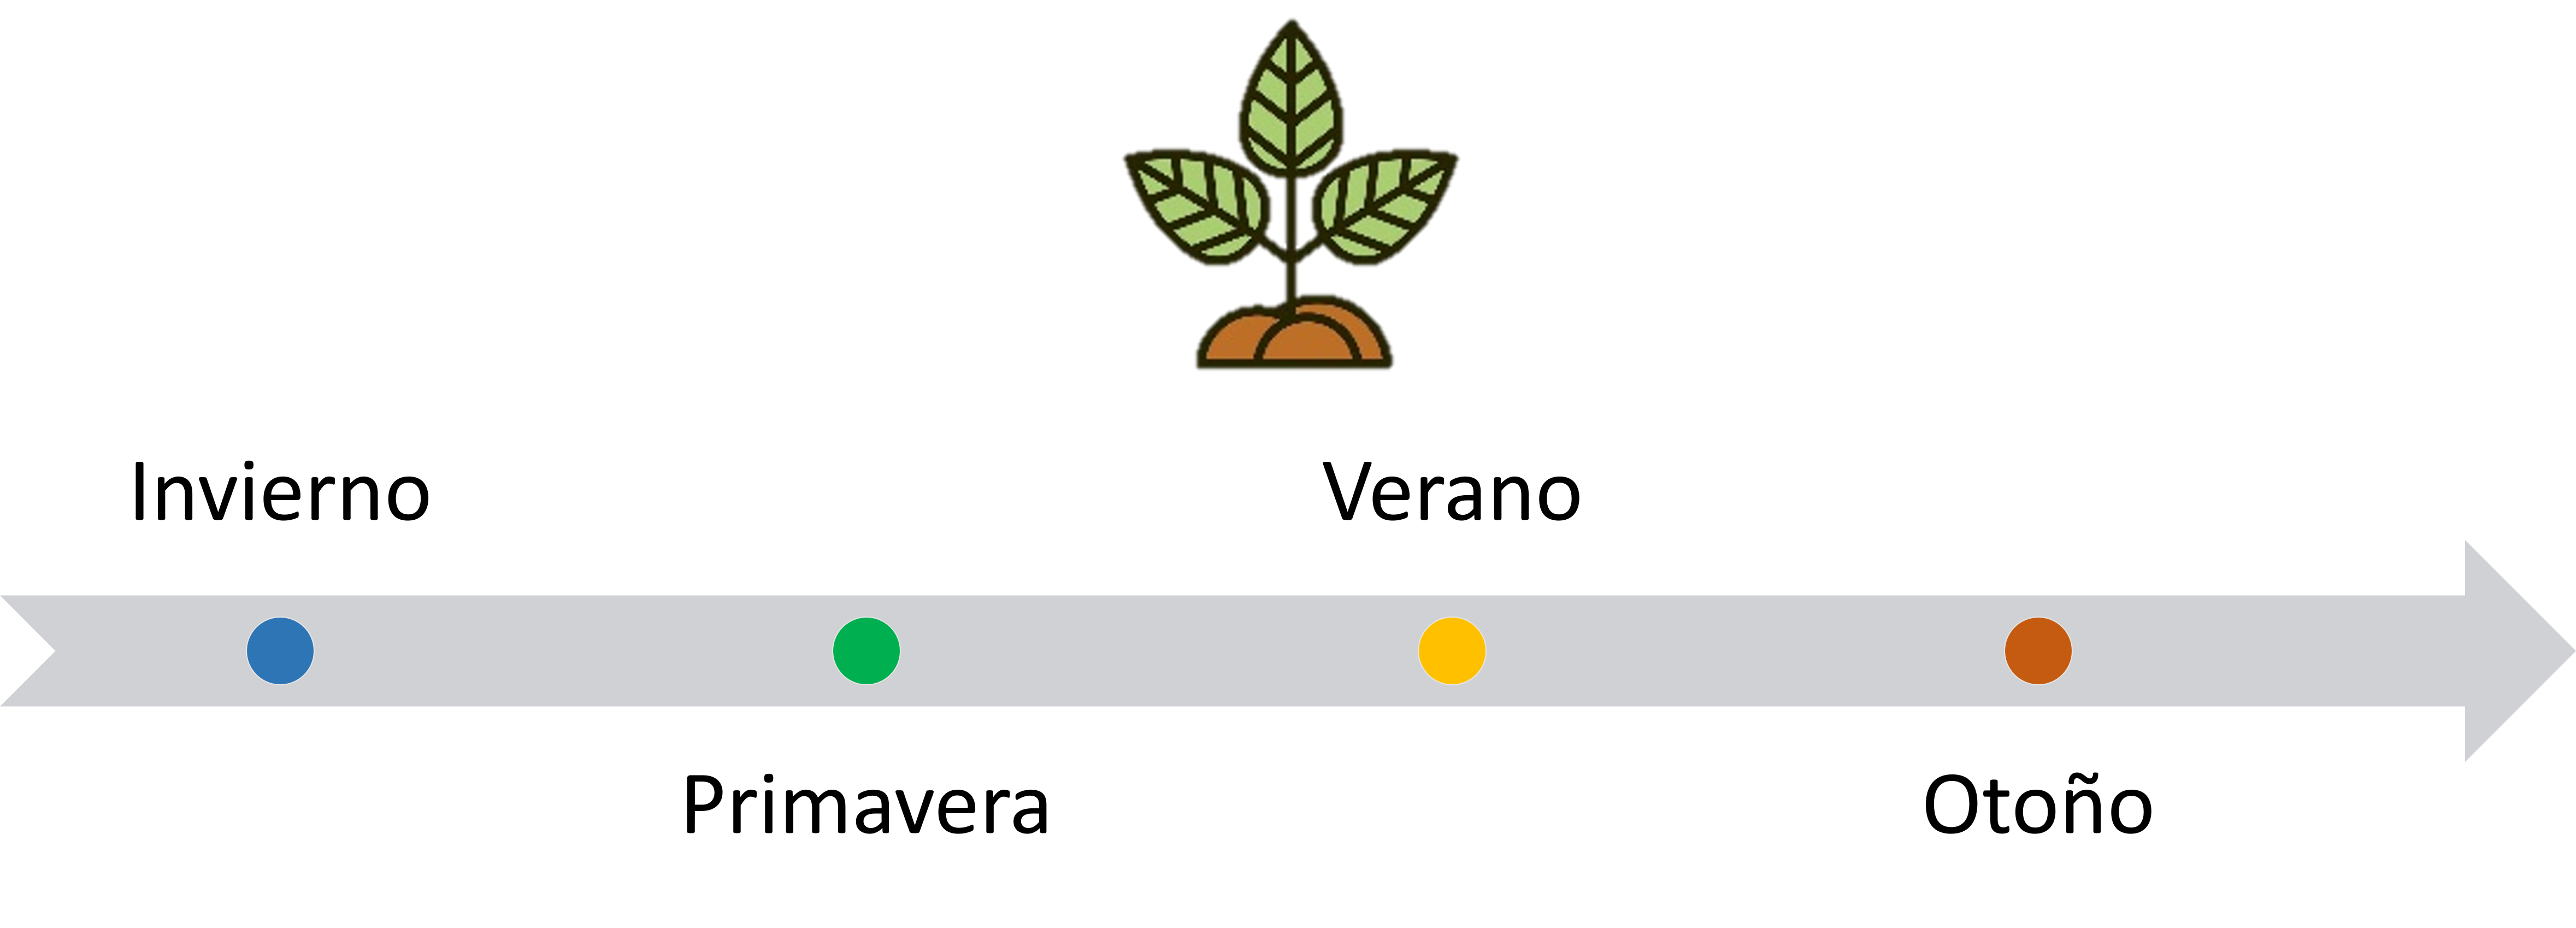
\includegraphics[width=\textwidth]{images/Choice.png}
\end{frame}

\begin{frame}{Motivación del problema}
	\vspace{-1cm}\centering
	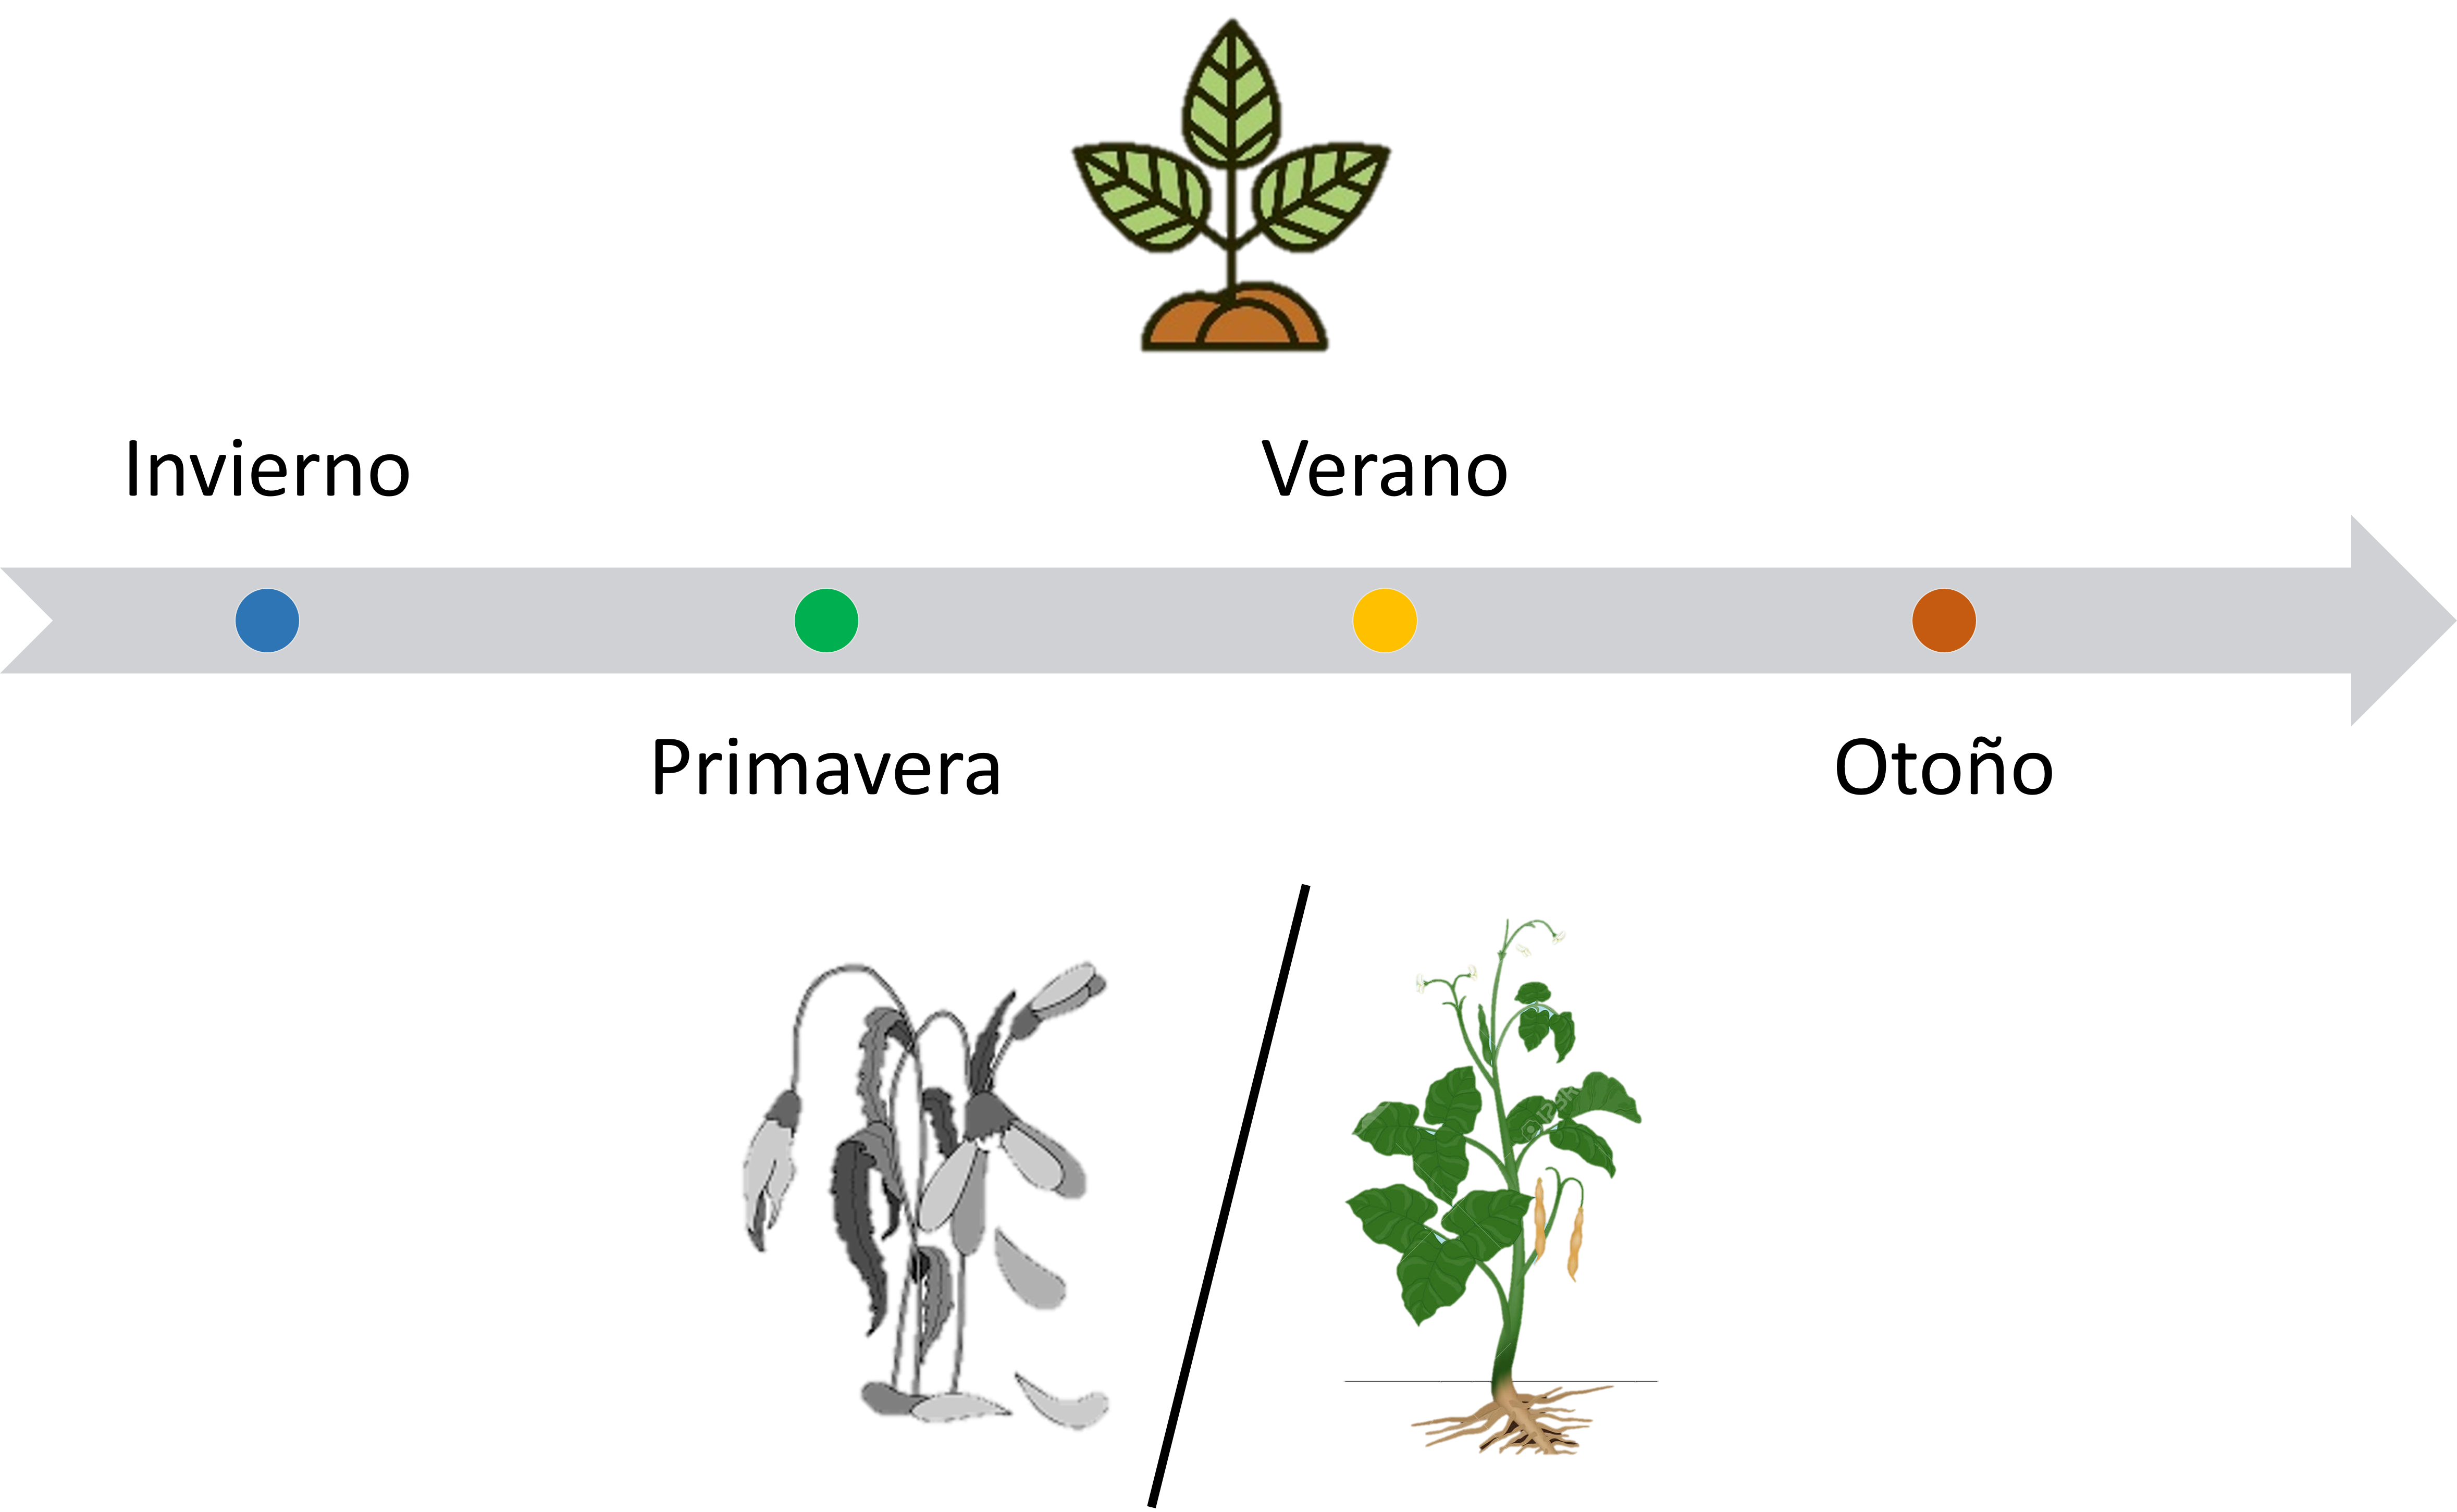
\includegraphics[width=0.9\textwidth]{images/Survival.png}
\end{frame}

\begin{frame}{Motivación del problema}
	 \vspace{-1cm}
	 \centering
	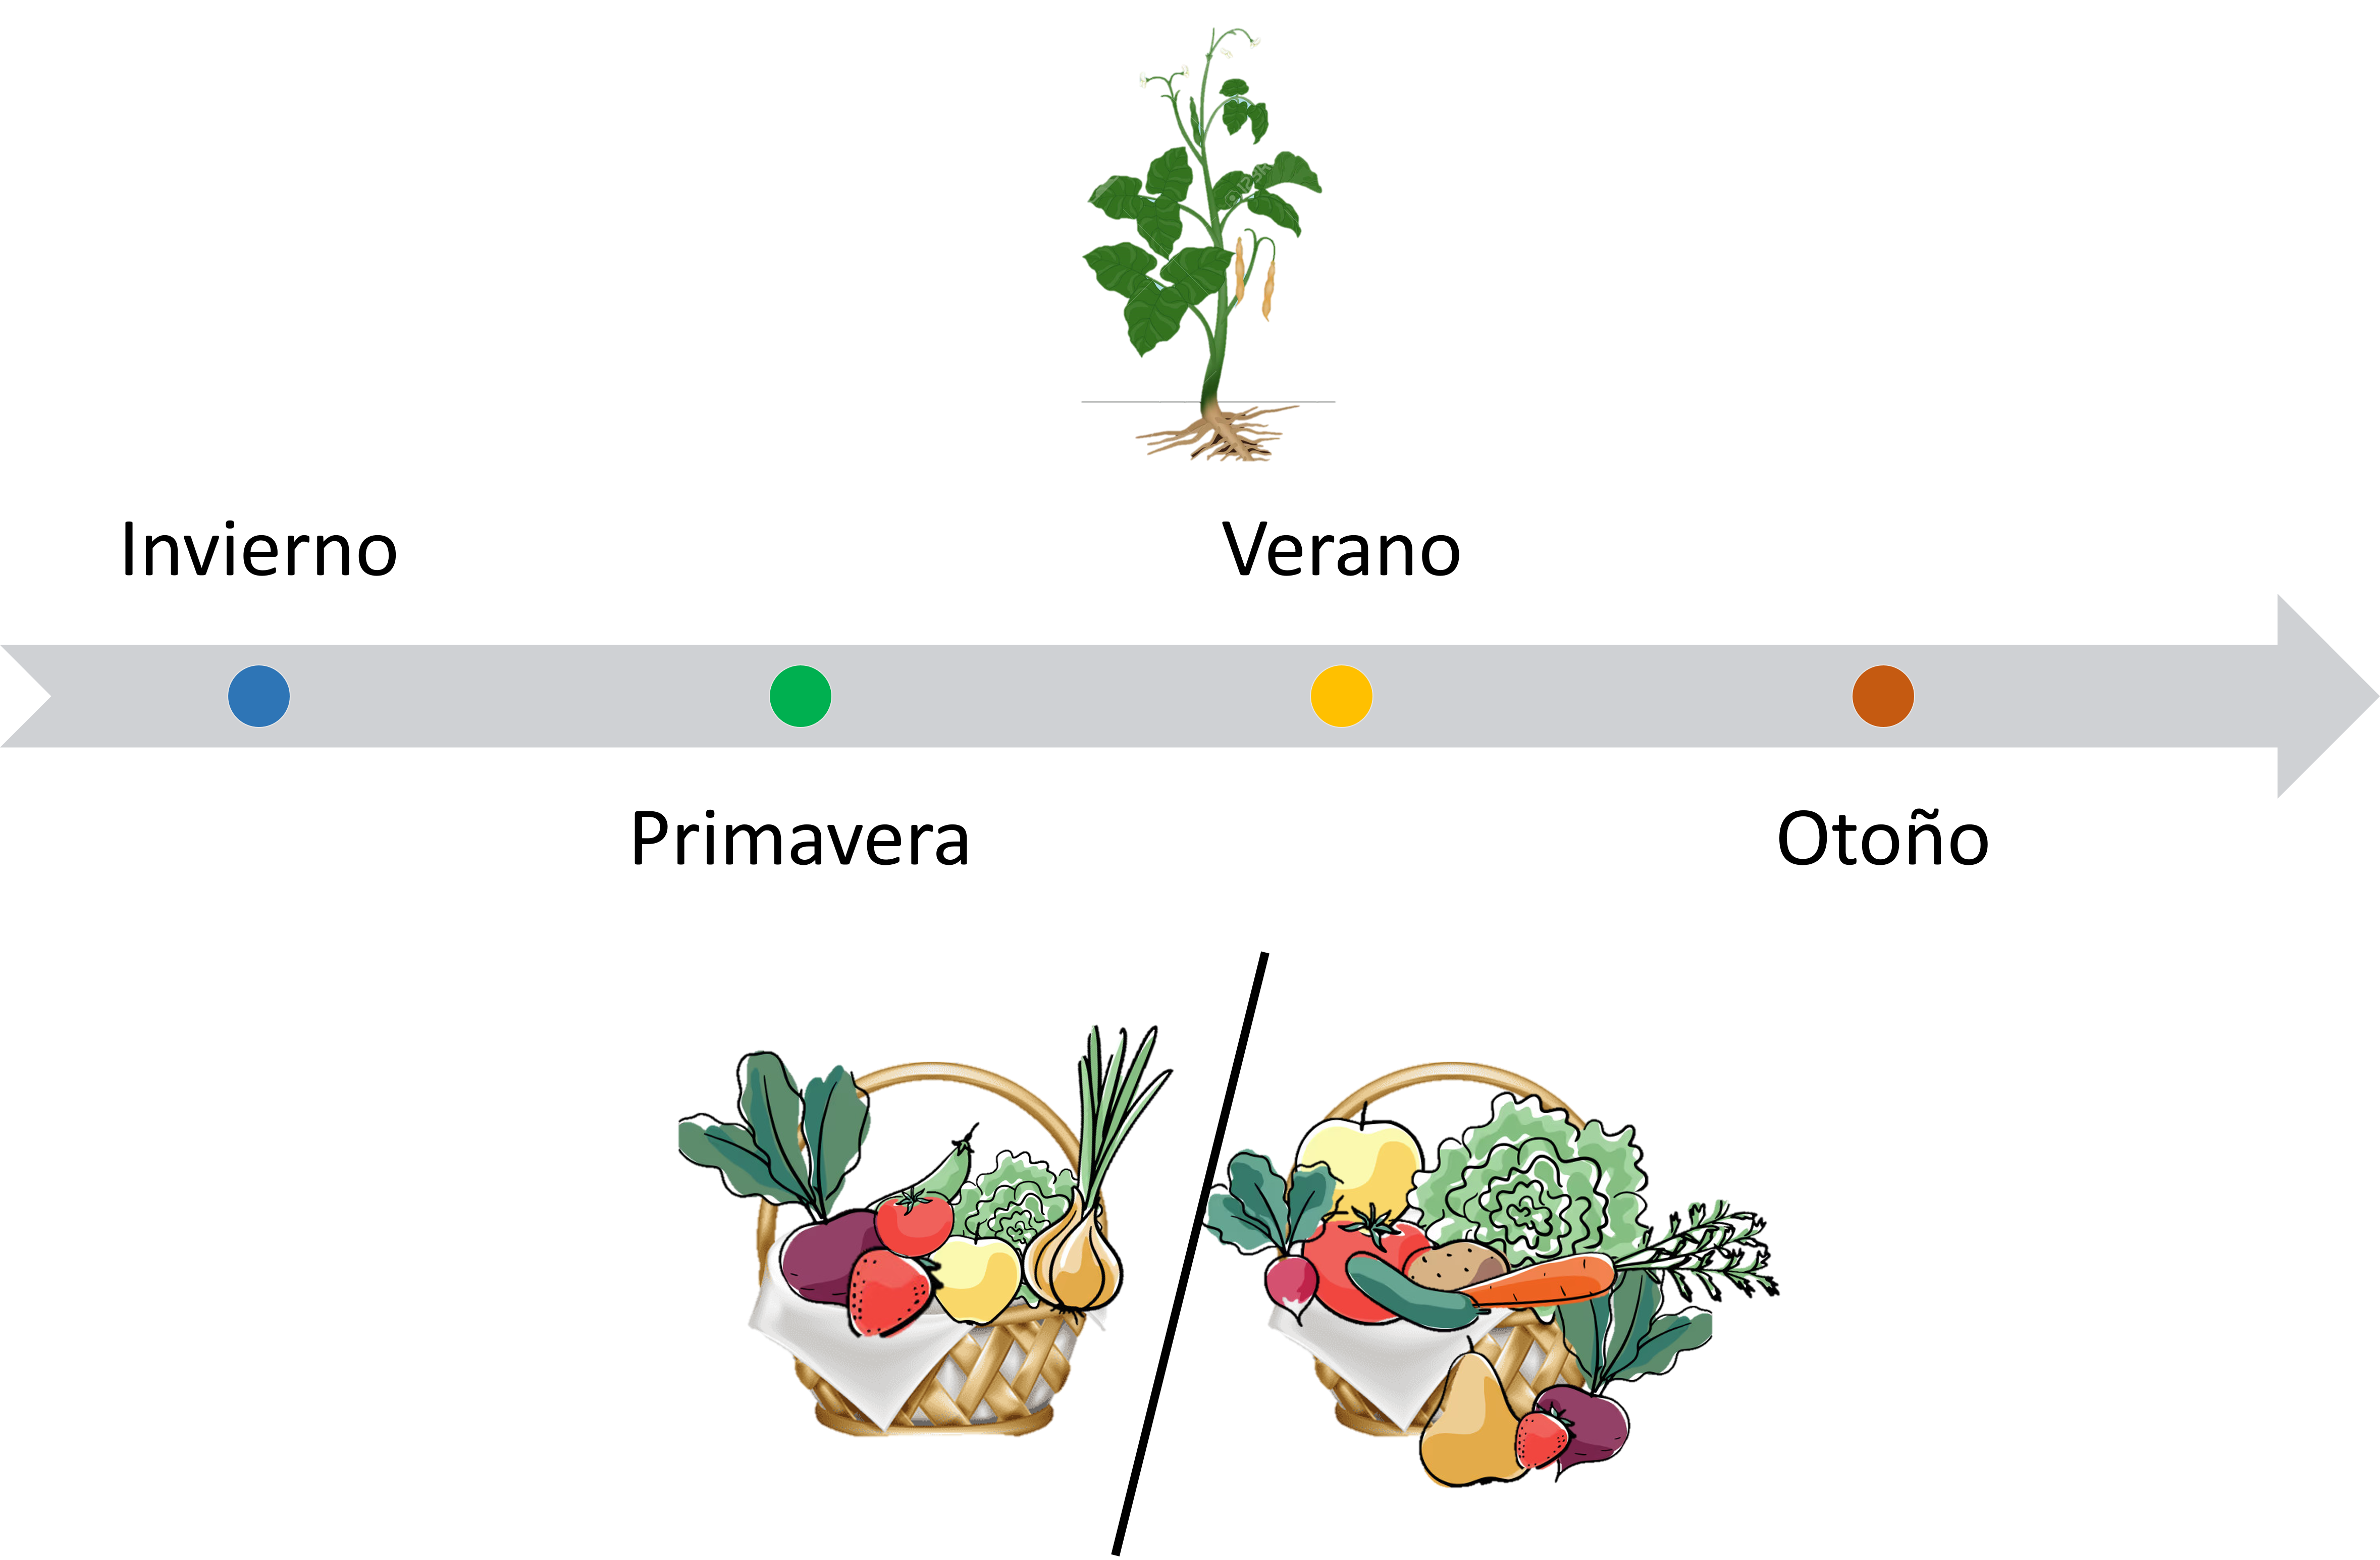
\includegraphics[width=0.9\textwidth]{images/Production.png}
\end{frame}

\begin{frame}{}
	\centering\Huge ¿Cómo determinar los periodos de siembra?
\end{frame}

\begin{frame}
	\vspace{-1cm}
	\centering
	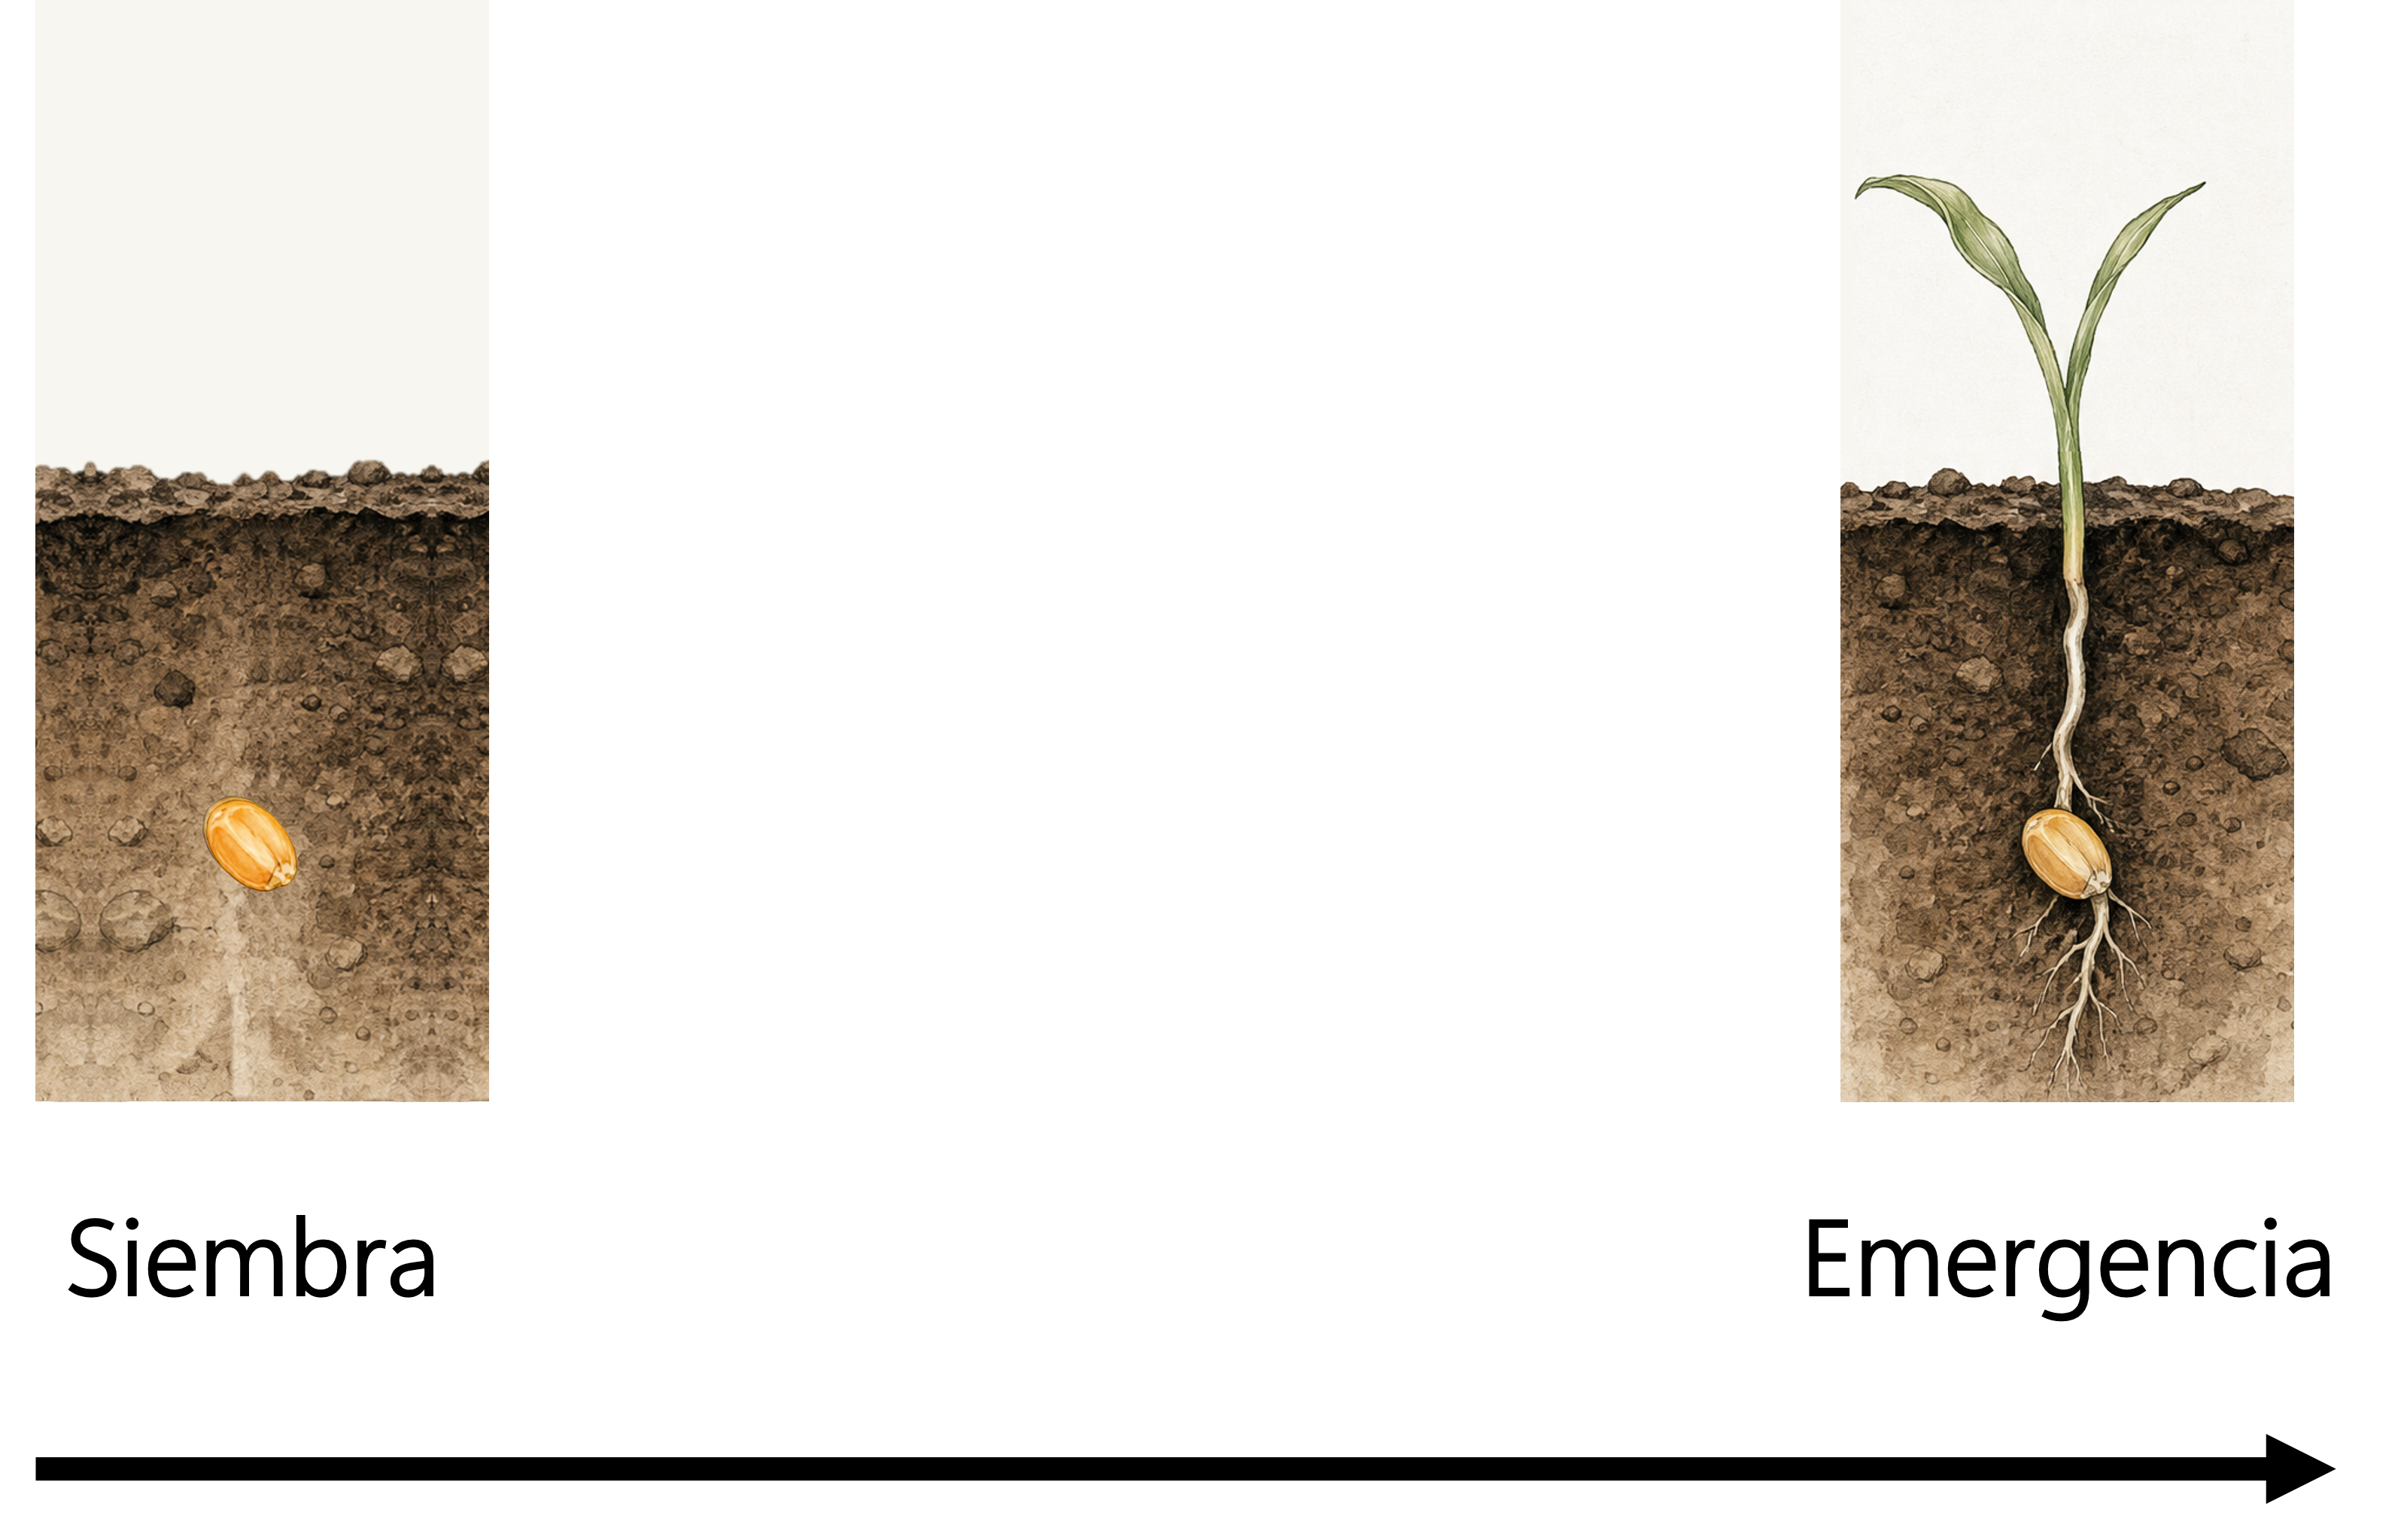
\includegraphics[width=0.9\textwidth]{images/Period.png}
	\pause $16.6 \pm 3.1$ días.\,\\
	\hfill \scriptsize Fuente: Chmielewski \textit{et al.} (2024); Sánchez \textit{et al.} (2013).
\end{frame}






\begin{frame}{Industria agrícola}
	\vspace{-1cm}
	\begin{minipage}{0.5\textwidth}
		\begin{block}{Estabilidad}
			\begin{itemize}
				\item Periodo luminoso.
				\item Temperaturas.
				\item Humedad.
				\item Características de suelo.
				\item Polinización.
				
			\end{itemize}
		\end{block}
	\end{minipage}%
	\begin{minipage}{0.5\textwidth}
		\pause\begin{block}{En ausencia}
			\begin{itemize}
				\item Problemas de seguridad alimentaria.
				\item Desequilibrio en la cadena trófica.
				\item Desabasto en industrias dependientes.
				\item Problemas económicos.
				\item Conflictos sociales.
			\end{itemize}
		\end{block}
	\end{minipage}
	\pause
	\centering
	\,\\ \Large
	En gran parte, las alteraciones pueden atribuirse al cambio climático.
\end{frame}


\begin{frame}{Impacto del cambio climático}
\vspace{-1cm}

\begin{block}{\centering Consecuencias}
       \begin{minipage}{0.5\textwidth}
			\begin{itemize}
				\item Estrés ambiental.
                \item Relaciones biológicas.
			\end{itemize}
		\end{minipage}%
		\begin{minipage}{0.5\textwidth}
			\begin{itemize}
				\item Escasez laboral.
                \item Volatilidad productiva.
			\end{itemize}
		\end{minipage}
    \end{block}
    \pause
    \begin{block}{Desfase de las estaciones del año \hfill {\scriptsize Fuente: Wang \textit{et al.} (2021).}}
    \centering
        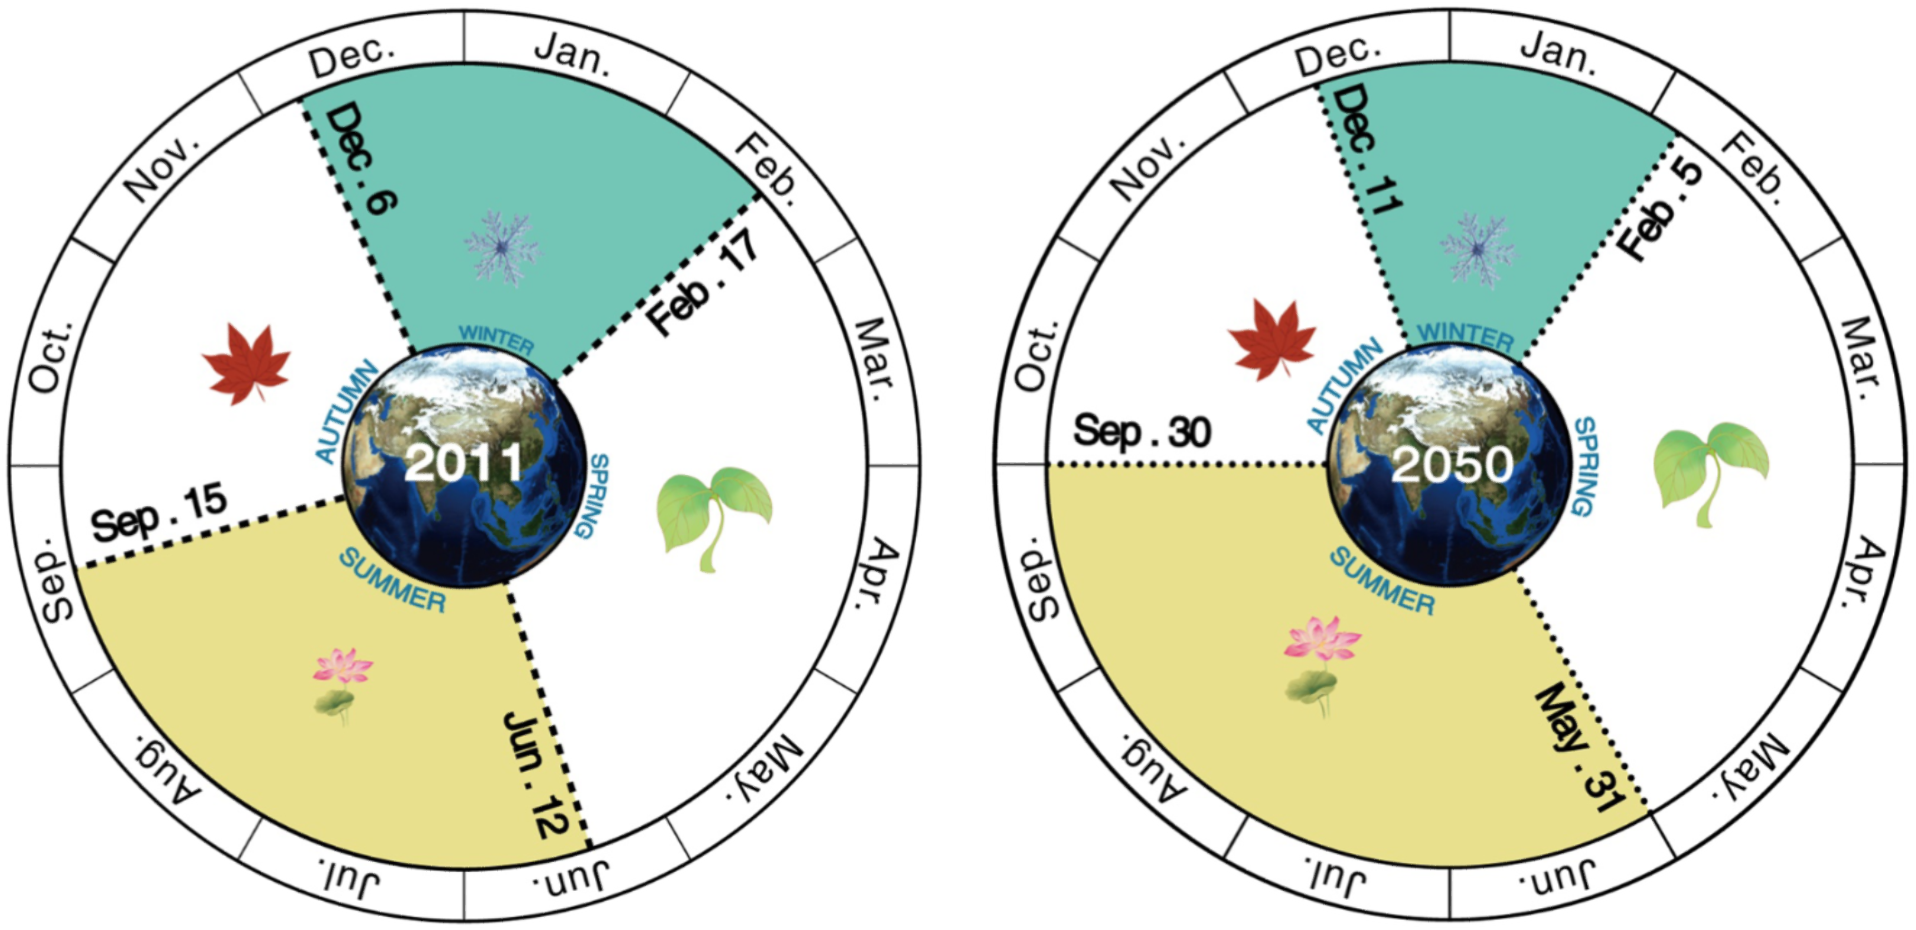
\includegraphics[scale=0.31]{images/Seasons.png}
    \end{block}
\end{frame}



\begin{frame}{Maíz}
	\vspace{-1cm}
		\begin{minipage}{0.5\textwidth}
			\vspace{-0.1cm}\begin{block}{}
				Usos
			\begin{itemize}
				\item Abastecimiento alimenticio.
				\item Medicamentos.
				\item Biocombustibles.
				\item Bebidas, jarabes, harinas y aceites.
			\end{itemize}
			\end{block}
			\pause\begin{block}{}
				Relevancia global
			\begin{itemize}
				\item Aporte calórico, proteico y graso.
				\item Producción superior 1100 millones de toneladas al año.
				\item Distribución geográfica asimétrica.
			\end{itemize}
			\end{block}
		\end{minipage}%
		\begin{minipage}{0.5\textwidth}
			\centering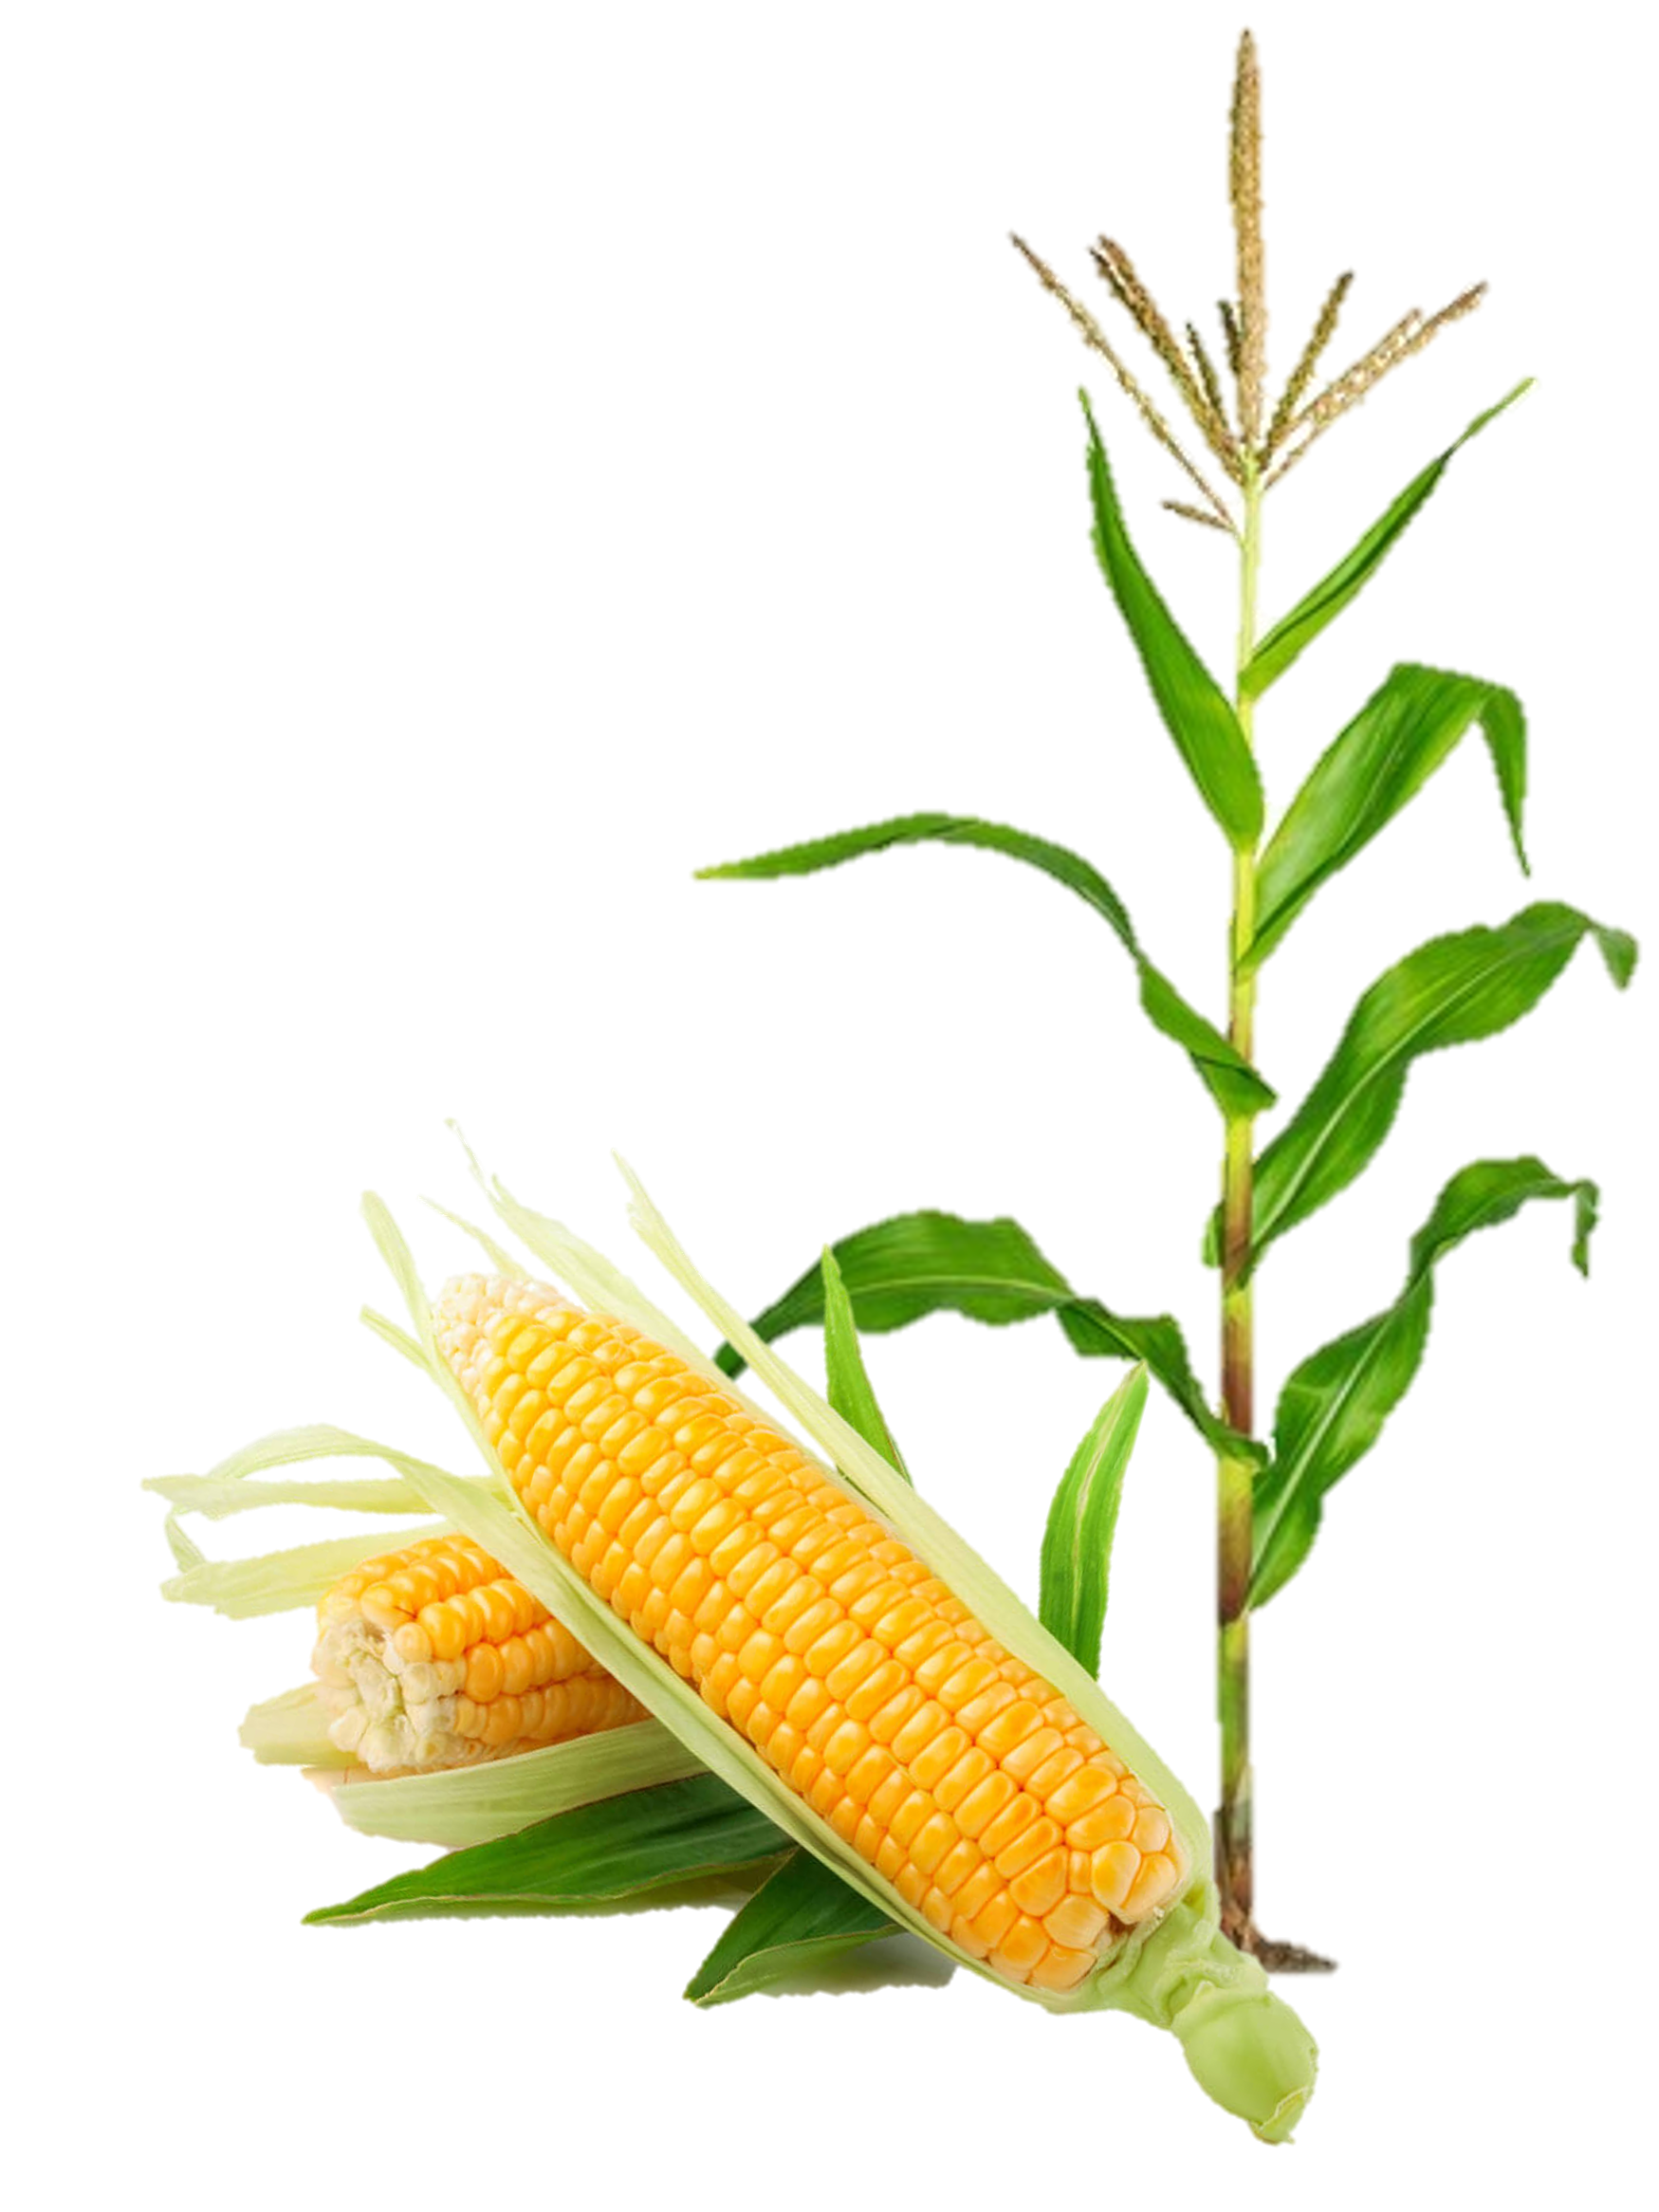
\includegraphics[height=0.8\textheight]{Maiz.png}
		\end{minipage}

		
\end{frame}

\begin{frame}{Maíz en Alemania}
	\vspace{-1cm}
	\begin{minipage}{0.5\textwidth}
		\centering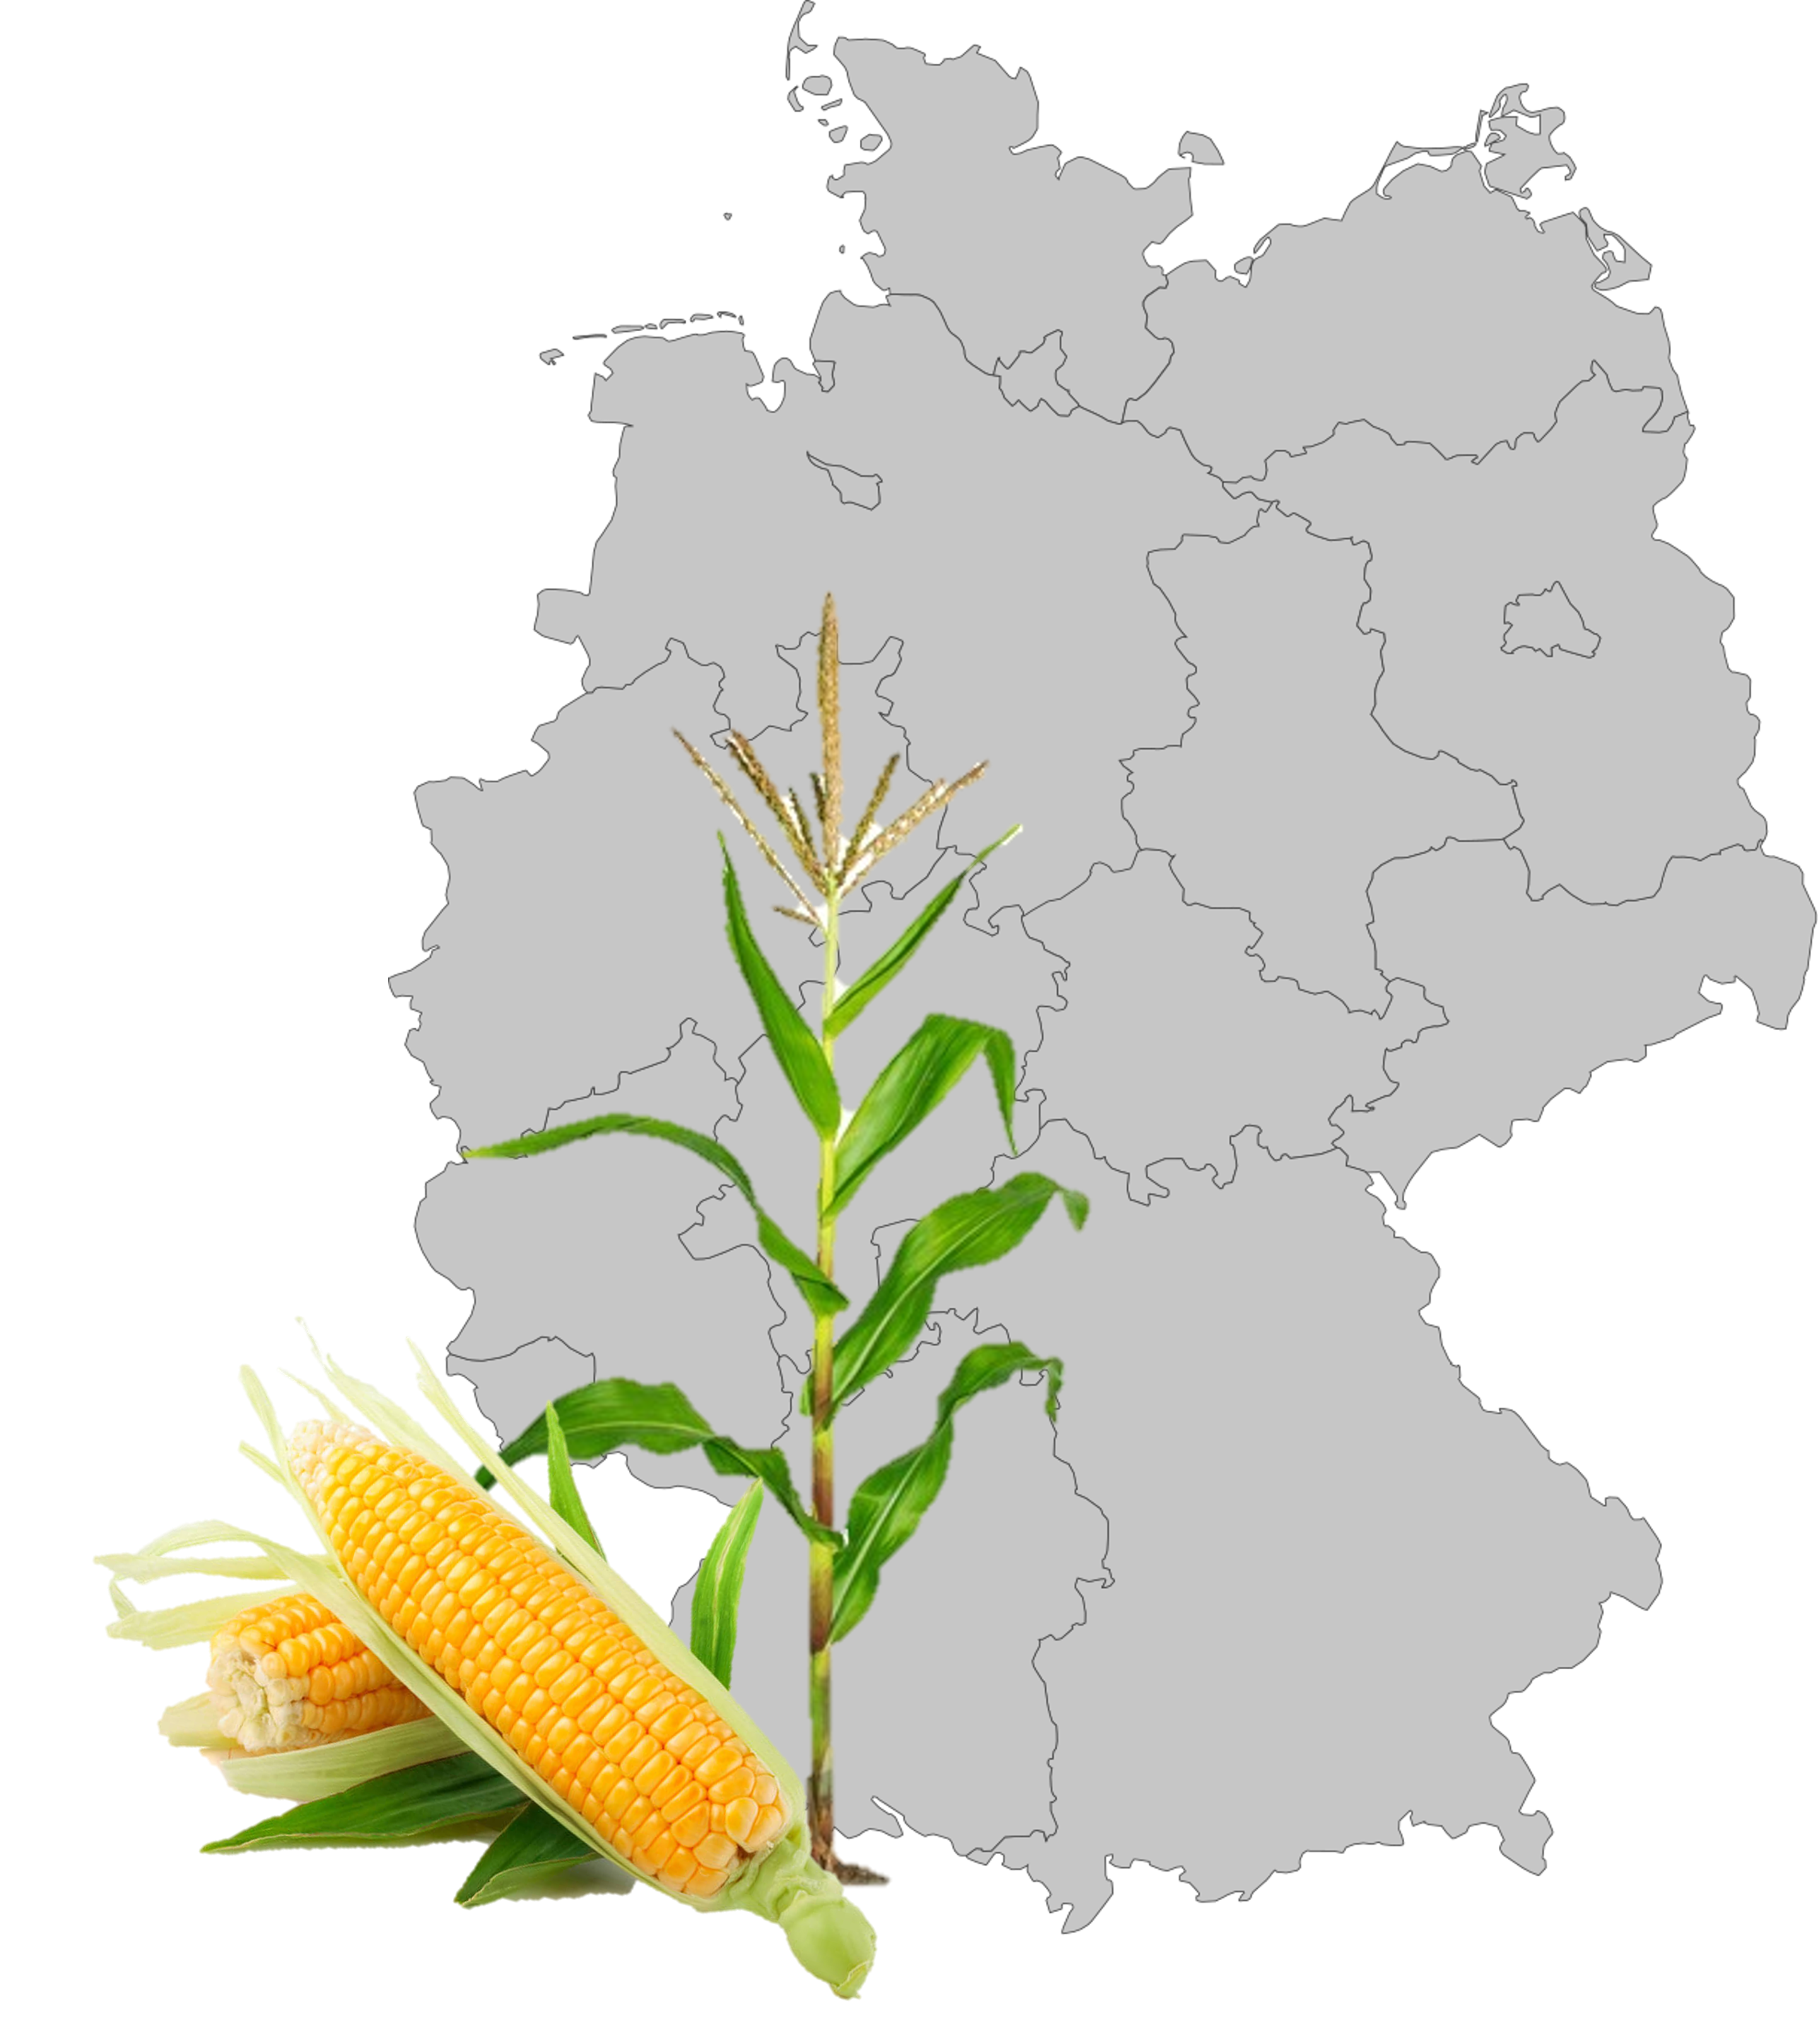
\includegraphics[height=0.8\textheight]{MaizGermany.png}
	\end{minipage}%
	\begin{minipage}{0.5\textwidth}
		\vspace{-0.1cm}\begin{block}{}
			Europa cuenta con el 8.91\% de las zonas de producción.\\
			\pause
			Alemania tendrá un incremento en
			las zonas con potencial de producción agrícola del maíz.
		\end{block}
		{\scriptsize Fuente: Miedaner \textit{et al.} (2021).}
	\end{minipage}%
\end{frame}



\section{Ante las alteraciones en los procesos agrícolas derivadas del cambio climático, ¿cómo predecir ventanas de siembra de maíz en Alemania mediante modelos probabilísticos empleando datos agroclimáticos más allá de los GDD?}


\begin{frame}{Objetivos generales}
	\vspace{-1.5cm}Desarrollar y validar un modelo probabilístico robusto, independiente de los GDD, que integre variables agroclimáticas significativas para predecir ventanas de fechas de siembra de maíz en el sureste de Alemania.
	\begin{minipage}{0.33\textwidth}
		\pause\begin{block}{Favorecer los ciclos de desarrollo}
		\end{block}
	\end{minipage}%
	\begin{minipage}{0.33\textwidth}
		\pause\begin{block}{Disminuir la exposición a estresores ambientales}
		\end{block}
	\end{minipage}%
	\begin{minipage}{0.33\textwidth}\pause\begin{block}{Contribuir a la toma de decisiones}
	\end{block}
	\end{minipage}
	\,\\
	\pause
	Contrastándolo con información oficial reportada para Alemania, un país con potencial agrícola en crecimiento debido a que se enfrenta a un contexto de transición climática derivado del cambio climático. 
\end{frame}



\begin{frame}{Datos agroclimáticos}
	\vspace{-1cm}
	\begin{columns}
		\column{0.40\textwidth}
		\begin{itemize}
			\item Temperatura ambiente promedio.
			\item Humedad relativa.
			\item Temperatura del suelo (5 cm de profundidad).
			\item Humedad del suelo (0 -- 10 cm de profundidad).
		\end{itemize}
		{\tiny Fuente: Deutscher Wetterdienst (2026); Climatic Research Unit (1997).}
		\column{0.60\textwidth}
		\begin{figure}[ht]
			\centering
			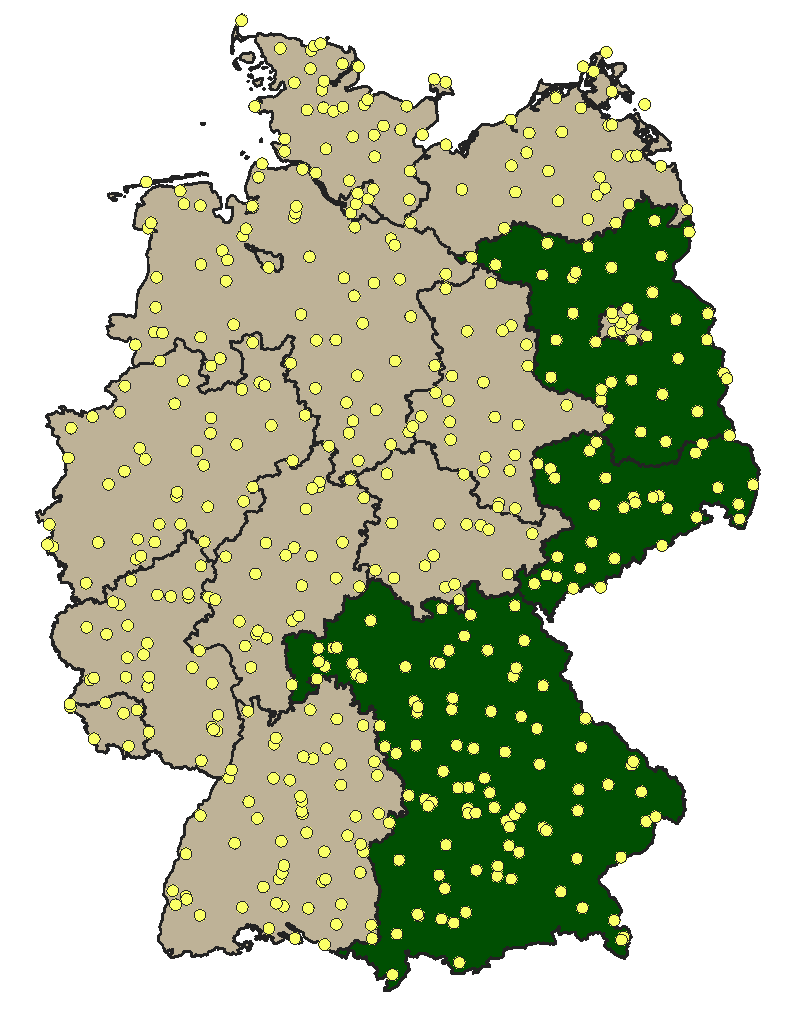
\includegraphics[height=0.8\textheight]{Stations per Federal State.pdf}
		\end{figure}
		\begin{center}
			\vspace{-0.5cm}
			{\tiny Total de 493 estaciones climáticas. Fuente: Deutscher Wetterdienst (2026).}
		\end{center}
	\end{columns}
\end{frame}





\begin{frame}{Modelo}
	\vspace{-0.8cm}
	\begin{figure}[ht]
		\centering
		%\shorthandoff{<>}
		\resizebox{0.6\textwidth}{!}{
			\begin{tikzpicture}[
				>=Stealth,
				state/.style={draw, circle, minimum size=14mm, line width=0.8pt},
				invisible/.style={circle, minimum size=14mm, draw=none},
				arrow/.style={->, line width=0.8pt}
				]
				
				% Centro
				\node[state] (F) at (0,0) {$F$};
				
				% Hexágono
				\node[state] (D1)   at (180:3.2cm) {$D_{1}$};
				\node[state] (D2)   at (240:3.2cm) {$D_{2}$};
				\node[invisible] (dots1) at (300:3.2cm) {};
				\node[state] (Di)   at (0:3.2cm) {$D_{i}$};
				\node[invisible] (dots2) at (60:3.2cm) {};
				\node[state] (D365) at (120:3.2cm) {$D_{365}$};
				
				% Ciclo
				\path[arrow]
				(D1) edge[bend right=15] 
				node[pos=0.3, sloped, below] {$\lambda_{1}$} (D2)
				
				(D2) edge[bend right=15] 
				node[pos=0.5, sloped, below] {$\lambda_{2}$} (dots1)
				
				(dots1) edge[bend right=15]
				node[pos=0.5, sloped, below] {$\lambda_{i-1}$} (Di)
				
				(Di) edge[bend right=15] 
				node[pos=0.4, sloped, above] {$\lambda_{i}$} (dots2)
				
				(dots2) edge[bend right=15]
				node[pos=0.5, sloped, above] {$\lambda_{364}$} (D365)
				
				(D365) edge[bend right=15] 
				node[pos=0.5, sloped, above] {$\lambda_{365}$} (D1);
				
				% Hacia F
				\path[arrow]
				(D1) edge node[pos=0.55,above] {$1-\lambda_{1}$} (F)
				(D2) edge node[pos=0.55, sloped, above] {$1-\lambda_{2}$} (F)
				(Di) edge node[pos=0.55, above] {$1-\lambda_{i}$} (F)
				(D365) edge node[pos=0.55, sloped, above] {$1-\lambda_{365}$} (F);
				
				% Loop
				\path[arrow]
				(F) edge[
				loop,
				out=320, 
				in=300,
				looseness=8
				] node[pos=0.8, xshift=10pt, yshift=-10pt] {$1$} (F);
				
				% Puntos suspensivos
				\node[font=\large, rotate=35] at (300:3.1cm) {$\cdots$};
				\node[font=\large, rotate=-30] at (60:3.1cm) {$\cdots$};
				
			\end{tikzpicture}
		}
		%\shorthandon{<>}
	\end{figure}
\end{frame}

\begin{frame}{Probabilidades de transición}
	\vspace{-0.7cm}
	\begin{figure}[ht]
		\centering
		\begin{tikzpicture}[x=0.75pt,y=0.75pt,yscale=-1,xscale=1]
			%uncomment if require: \path (0,717); %set diagram left start at 0, and has height of 717
			
			%Shape: Axis 2D [id:dp4496072713140289] 
			\draw  (58,700.13) -- (550,700.13)(64.03,422.4) -- (64.03,706.4) (540,695.13) -- (550,700.13) -- (540,705.13) (59.03,432.4) -- (64.03,422.4) -- (69.03,432.4)  ;
			%Shape: Circle [id:dp06215554504361531] 
			\draw  [fill={rgb, 255:red, 0; green, 0; blue, 0 }  ,fill opacity=1 ] (133.6,481.2) .. controls (133.6,478.88) and (135.48,477) .. (137.8,477) .. controls (140.12,477) and (142,478.88) .. (142,481.2) .. controls (142,483.52) and (140.12,485.4) .. (137.8,485.4) .. controls (135.48,485.4) and (133.6,483.52) .. (133.6,481.2) -- cycle ;
			%Shape: Circle [id:dp22652234947291816] 
			\draw  [fill={rgb, 255:red, 0; green, 0; blue, 0 }  ,fill opacity=1 ] (182.6,481.2) .. controls (182.6,478.88) and (184.48,477) .. (186.8,477) .. controls (189.12,477) and (191,478.88) .. (191,481.2) .. controls (191,483.52) and (189.12,485.4) .. (186.8,485.4) .. controls (184.48,485.4) and (182.6,483.52) .. (182.6,481.2) -- cycle ;
			%Shape: Circle [id:dp7411954551562622] 
			\draw  [fill={rgb, 255:red, 0; green, 0; blue, 0 }  ,fill opacity=1 ] (172.6,447.26) .. controls (172.6,444.98) and (174.45,443.13) .. (176.74,443.13) .. controls (179.02,443.13) and (180.87,444.98) .. (180.87,447.26) .. controls (180.87,449.55) and (179.02,451.4) .. (176.74,451.4) .. controls (174.45,451.4) and (172.6,449.55) .. (172.6,447.26) -- cycle ;
			%Shape: Circle [id:dp9342194323542646] 
			\draw  [fill={rgb, 255:red, 0; green, 0; blue, 0 }  ,fill opacity=1 ] (110.6,481.2) .. controls (110.6,478.88) and (112.48,477) .. (114.8,477) .. controls (117.12,477) and (119,478.88) .. (119,481.2) .. controls (119,483.52) and (117.12,485.4) .. (114.8,485.4) .. controls (112.48,485.4) and (110.6,483.52) .. (110.6,481.2) -- cycle ;
			%Shape: Circle [id:dp7509634202671536] 
			\draw  [fill={rgb, 255:red, 0; green, 0; blue, 0 }  ,fill opacity=1 ] (130.6,517.2) .. controls (130.6,514.88) and (132.48,513) .. (134.8,513) .. controls (137.12,513) and (139,514.88) .. (139,517.2) .. controls (139,519.52) and (137.12,521.4) .. (134.8,521.4) .. controls (132.48,521.4) and (130.6,519.52) .. (130.6,517.2) -- cycle ;
			%Shape: Circle [id:dp3389656361514962] 
			\draw  [fill={rgb, 255:red, 0; green, 0; blue, 0 }  ,fill opacity=1 ] (119.6,497.2) .. controls (119.6,494.88) and (121.48,493) .. (123.8,493) .. controls (126.12,493) and (128,494.88) .. (128,497.2) .. controls (128,499.52) and (126.12,501.4) .. (123.8,501.4) .. controls (121.48,501.4) and (119.6,499.52) .. (119.6,497.2) -- cycle ;
			%Shape: Circle [id:dp7223141295117336] 
			\draw  [fill={rgb, 255:red, 0; green, 0; blue, 0 }  ,fill opacity=1 ] (149.6,512.2) .. controls (149.6,509.88) and (151.48,508) .. (153.8,508) .. controls (156.12,508) and (158,509.88) .. (158,512.2) .. controls (158,514.52) and (156.12,516.4) .. (153.8,516.4) .. controls (151.48,516.4) and (149.6,514.52) .. (149.6,512.2) -- cycle ;
			%Shape: Circle [id:dp7582728872550809] 
			\draw  [fill={rgb, 255:red, 0; green, 0; blue, 0 }  ,fill opacity=1 ] (116.6,454.2) .. controls (116.6,451.88) and (118.48,450) .. (120.8,450) .. controls (123.12,450) and (125,451.88) .. (125,454.2) .. controls (125,456.52) and (123.12,458.4) .. (120.8,458.4) .. controls (118.48,458.4) and (116.6,456.52) .. (116.6,454.2) -- cycle ;
			%Shape: Circle [id:dp49904732080555536] 
			\draw  [fill={rgb, 255:red, 0; green, 0; blue, 0 }  ,fill opacity=1 ] (163.6,506.2) .. controls (163.6,503.88) and (165.48,502) .. (167.8,502) .. controls (170.12,502) and (172,503.88) .. (172,506.2) .. controls (172,508.52) and (170.12,510.4) .. (167.8,510.4) .. controls (165.48,510.4) and (163.6,508.52) .. (163.6,506.2) -- cycle ;
			%Shape: Circle [id:dp9713308312029804] 
			\draw  [fill={rgb, 255:red, 0; green, 0; blue, 0 }  ,fill opacity=1 ] (164.6,486.2) .. controls (164.6,483.88) and (166.48,482) .. (168.8,482) .. controls (171.12,482) and (173,483.88) .. (173,486.2) .. controls (173,488.52) and (171.12,490.4) .. (168.8,490.4) .. controls (166.48,490.4) and (164.6,488.52) .. (164.6,486.2) -- cycle ;
			%Shape: Circle [id:dp6213316985023771] 
			\draw  [fill={rgb, 255:red, 0; green, 0; blue, 0 }  ,fill opacity=1 ] (164.6,520.2) .. controls (164.6,517.88) and (166.48,516) .. (168.8,516) .. controls (171.12,516) and (173,517.88) .. (173,520.2) .. controls (173,522.52) and (171.12,524.4) .. (168.8,524.4) .. controls (166.48,524.4) and (164.6,522.52) .. (164.6,520.2) -- cycle ;
			%Shape: Polygon [id:ds0377823447882647] 
			\draw [fill={rgb, 255:red, 20; green, 20; blue, 80 }  ,fill opacity=0.25 ] (452,517.2) -- (496,551.8) -- (452,627.2) -- (422,607.2) -- (408,542.8) -- cycle ;
			%Flowchart: Summing Junction [id:dp4210872697663528] 
			\draw  [fill={rgb, 255:red, 74; green, 144; blue, 226 }  ,fill opacity=1 ][line width=0.5]  (147,488.6) .. controls (147,486.06) and (149.24,484) .. (152,484) .. controls (154.76,484) and (157,486.06) .. (157,488.6) .. controls (157,491.14) and (154.76,493.2) .. (152,493.2) .. controls (149.24,493.2) and (147,491.14) .. (147,488.6) -- cycle ;% \draw  [line width=1.5]  (148.46,485.35) -- (155.54,491.85) ; \draw  [line width=1.5]  (155.54,485.35) -- (148.46,491.85) ;
			%Shape: Circle [id:dp3856640767966395] 
			\draw  [fill={rgb, 255:red, 0; green, 0; blue, 0 }  ,fill opacity=1 ] (137.6,504.2) .. controls (137.6,501.88) and (139.48,500) .. (141.8,500) .. controls (144.12,500) and (146,501.88) .. (146,504.2) .. controls (146,506.52) and (144.12,508.4) .. (141.8,508.4) .. controls (139.48,508.4) and (137.6,506.52) .. (137.6,504.2) -- cycle ;
			%Flowchart: Summing Junction [id:dp21052777836013448] 
			\draw  [fill={rgb, 255:red, 208; green, 2; blue, 27 }  ,fill opacity=1 ][line width=0.5]  (444,572.6) .. controls (444,570.06) and (446.24,568) .. (449,568) .. controls (451.76,568) and (454,570.06) .. (454,572.6) .. controls (454,575.14) and (451.76,577.2) .. (449,577.2) .. controls (446.24,577.2) and (444,575.14) .. (444,572.6) -- cycle ; %\draw  [line width=1.5]  (445.46,569.35) -- (452.54,575.85) ; \draw  [line width=1.5]  (452.54,569.35) -- (445.46,575.85) ;
			%Straight Lines [id:da05984024528227749] 
			\draw  [dash pattern={on 4.5pt off 4.5pt}]  (157,490.6) -- (444,572.6) ;
			%Shape: Circle [id:dp618933165821857] 
			\draw  [fill={rgb, 255:red, 0; green, 0; blue, 0 }  ,fill opacity=1 ] (146.6,453.2) .. controls (146.6,450.88) and (148.48,449) .. (150.8,449) .. controls (153.12,449) and (155,450.88) .. (155,453.2) .. controls (155,455.52) and (153.12,457.4) .. (150.8,457.4) .. controls (148.48,457.4) and (146.6,455.52) .. (146.6,453.2) -- cycle ;
			
			% Text Node
			\draw (104,534.4) node [anchor=north west][inner sep=0.75pt]  [font=\small] [align=left] {\begin{minipage}[lt]{85.87pt}\setlength\topsep{0pt}
					\begin{center}
						Historical data\\from the $k$-th day
					\end{center}
					
			\end{minipage}};
			% Text Node
			\draw (393,637.4) node [anchor=north west][inner sep=0.75pt]  [font=\small] [align=left] {\begin{minipage}[lt]{78.21pt}\setlength\topsep{0pt}
					\begin{center}
						Optimal conditions
					\end{center}
					
			\end{minipage}};
			% Text Node
			\draw (136.6,460.6) node [anchor=north west][inner sep=0.75pt]    {$C_{H,k}$};
			% Text Node
			\draw (436,544.4) node [anchor=north west][inner sep=0.75pt]    {$C^*$};
			\draw (257,475.8) node [anchor=north west][inner sep=0.75pt]    {$d( C_{H,k} \ \mathbf{,}\ C^*)$};
			% Text Node
			\draw (110,600.4) node [anchor=north west, font=\Large][inner sep=0.75pt] {
				$\displaystyle 
				\lambda_k := 1 - \frac{d(C_{H,k}\,,\, C^*)}{\displaystyle\max_{l\in \{1,\dots,365\}} \{d(C_{H,l}\,,\, C^*)\}}.$
			};
		\end{tikzpicture}
	\end{figure}
\end{frame}





\begin{frame}{Modelo: Criterio  empírico de permanencia}
	\vspace{-0.7cm}
	\begin{columns}
		\column{0.5\textwidth}
		\begin{figure}[ht]
			\centering
			%\shorthandoff{<>}
			\resizebox{\textwidth}{!}{
				\begin{tikzpicture}[
					>=Stealth,
					state/.style={draw, circle, minimum size=14mm, line width=0.8pt},
					invisible/.style={circle, minimum size=14mm, draw=none},
					arrow/.style={->, line width=0.8pt}
					]
					
					% Centro
					\node[state] (F) at (0,0) {$F$};
					
					% Hexágono
					\node[state] (D1)   at (180:3.2cm) {$D_{1}$};
					\node[state] (D2)   at (240:3.2cm) {$D_{2}$};
					\node[invisible] (dots1) at (300:3.2cm) {};
					\node[state] (Di)   at (0:3.2cm) {$D_{i}$};
					\node[invisible] (dots2) at (60:3.2cm) {};
					\node[state] (D365) at (120:3.2cm) {$D_{365}$};
					
					% Ciclo
					\path[arrow]
					(D1) edge[bend right=15] 
					node[pos=0.3, sloped, below] {$\lambda_{1}$} (D2)
					
					(D2) edge[bend right=15] 
					node[pos=0.5, sloped, below] {$\lambda_{2}$} (dots1)
					
					(dots1) edge[bend right=15]
					node[pos=0.5, sloped, below] {$\lambda_{i-1}$} (Di)
					
					(Di) edge[bend right=15] 
					node[pos=0.4, sloped, above] {$\lambda_{i}$} (dots2)
					
					(dots2) edge[bend right=15]
					node[pos=0.5, sloped, above] {$\lambda_{364}$} (D365)
					
					(D365) edge[bend right=15] 
					node[pos=0.5, sloped, above] {$\lambda_{365}$} (D1);
					
					% Hacia F
					\path[arrow]
					(D1) edge node[pos=0.55,above] {$1-\lambda_{1}$} (F)
					(D2) edge node[pos=0.55, sloped, above] {$1-\lambda_{2}$} (F)
					(Di) edge node[pos=0.55, above] {$1-\lambda_{i}$} (F)
					(D365) edge node[pos=0.55, sloped, above] {$1-\lambda_{365}$} (F);
					
					% Loop
					\path[arrow]
					(F) edge[
					loop,
					out=320, 
					in=300,
					looseness=8
					] node[pos=0.8, xshift=10pt, yshift=-10pt] {$1$} (F);
					
					% Puntos suspensivos
					\node[font=\large, rotate=35] at (300:3.1cm) {$\cdots$};
					\node[font=\large, rotate=-30] at (60:3.1cm) {$\cdots$};
					
				\end{tikzpicture}
			}
			%\shorthandon{<>}
		\end{figure}
		\column{0.5\textwidth}
		Calcular
		$$P_i(\tau_F > n^*):=P(\tau_F > n^*\mid X_0=D_i),$$ con $\displaystyle\{\tau_F > n^*\}= \inf_{t\in \mathbb{N}} \{X_t= F\}.$\\
		\begin{block}{Metodología de de Anda-Jauregui \textit{et al.} (2021).}
			Por realizar $r^*\in  \mathbb{N}$ caminatas aleatorias
			$$\widehat{P_i}(\tau_F > n^*):=\frac{|W(D_{i}, D_{(i+n^*)\bmod{365}})|}{r^*} \geq \zeta^*.$$
		\end{block}
		Intervalos de $(1-\alpha)100\%$ de confianza por bootstrap y jackknife.
	\end{columns}
\end{frame}




\begin{frame}{Cadena de Markov absorbente}
	\vspace{-0.7cm}
	\begin{columns}
		\column{0.4\textwidth}
		\begin{figure}[ht]
			\centering
			%\shorthandoff{<>}
			\resizebox{1.2\textwidth}{!}{
				\begin{tikzpicture}[
					>=Stealth,
					state/.style={draw, circle, minimum size=14mm, line width=0.8pt},
					invisible/.style={circle, minimum size=14mm, draw=none},
					arrow/.style={->, line width=0.8pt}
					]
					
					% Centro
					\node[state] (F) at (0,0) {$F$};
					
					% Hexágono
					\node[state] (D1)   at (180:3.2cm) {$D_{1}$};
					\node[state] (D2)   at (240:3.2cm) {$D_{2}$};
					\node[invisible] (dots1) at (300:3.2cm) {};
					\node[state] (Di)   at (0:3.2cm) {$D_{i}$};
					\node[invisible] (dots2) at (60:3.2cm) {};
					\node[state] (D365) at (120:3.2cm) {$D_{365}$};
					
					% Ciclo
					\path[arrow]
					(D1) edge[bend right=15] 
					node[pos=0.3, sloped, below] {$\lambda_{1}$} (D2)
					
					(D2) edge[bend right=15] 
					node[pos=0.5, sloped, below] {$\lambda_{2}$} (dots1)
					
					(dots1) edge[bend right=15]
					node[pos=0.5, sloped, below] {$\lambda_{i-1}$} (Di)
					
					(Di) edge[bend right=15] 
					node[pos=0.4, sloped, above] {$\lambda_{i}$} (dots2)
					
					(dots2) edge[bend right=15]
					node[pos=0.5, sloped, above] {$\lambda_{364}$} (D365)
					
					(D365) edge[bend right=15] 
					node[pos=0.5, sloped, above] {$\lambda_{365}$} (D1);
					
					% Hacia F
					\path[arrow]
					(D1) edge node[pos=0.55,above] {$1-\lambda_{1}$} (F)
					(D2) edge node[pos=0.55, sloped, above] {$1-\lambda_{2}$} (F)
					(Di) edge node[pos=0.55, above] {$1-\lambda_{i}$} (F)
					(D365) edge node[pos=0.55, sloped, above] {$1-\lambda_{365}$} (F);
					
					% Loop
					\path[arrow]
					(F) edge[
					loop,
					out=320, 
					in=300,
					looseness=8
					] node[pos=0.8, xshift=10pt, yshift=-10pt] {$1$} (F);
					
					% Puntos suspensivos
					\node[font=\large, rotate=35] at (300:3.1cm) {$\cdots$};
					\node[font=\large, rotate=-30] at (60:3.1cm) {$\cdots$};
					
				\end{tikzpicture}
			}
			%\shorthandon{<>}
		\end{figure}
		\column{0.7\textwidth}
		
		\begin{equation*}
			\phantom{A=}\begin{bNiceMatrix}[%
				first-row, 
				first-col]
				& D_1 & D_2 &D_3& D_4&\cdots &D_{364}&D_{365}&F \\
				D_1 & 0 & \lambda_1  &0  &0 & \cdots &0& 0 & 1-\lambda_1\\
				D_2 & 0 & 0  &\lambda_2  &0 & \cdots &0& 0 & 1-\lambda_2\\
				&&&&&&&\\
				\vdots\phantom{d} &&&&&\ddots&&&\vdots\\
				&&&&&&&\\
				D_{364} & 0 & 0  &0 &0 & \cdots &0& \lambda_{364}  & 1-\lambda_{364}\\
				D_{365} & \lambda_{365}   & 0  &0 &0 & \cdots &0& 0 & 1-\lambda_{365}\\
				F& 0  & 0  &0 &0 & \cdots &0& 0 & 1
			\end{bNiceMatrix}
		\end{equation*}
	\end{columns}
\end{frame}

\begin{frame}{Cadena de Markov absorbente}
	\vspace{-0.7cm}
	\begin{columns}
		\column{0.4\textwidth}
		\begin{figure}[ht]
			\centering
			%\shorthandoff{<>}
			\resizebox{1.2\textwidth}{!}{
				\begin{tikzpicture}[
					>=Stealth,
					state/.style={draw, circle, minimum size=14mm, line width=0.8pt},
					invisible/.style={circle, minimum size=14mm, draw=none},
					arrow/.style={->, line width=0.8pt}
					]
					
					% Centro
					\node[state] (F) at (0,0) {$F$};
					
					% Hexágono
					\node[state] (D1)   at (180:3.2cm) {$D_{1}$};
					\node[state] (D2)   at (240:3.2cm) {$D_{2}$};
					\node[invisible] (dots1) at (300:3.2cm) {};
					\node[state] (Di)   at (0:3.2cm) {$D_{i}$};
					\node[invisible] (dots2) at (60:3.2cm) {};
					\node[state] (D365) at (120:3.2cm) {$D_{365}$};
					
					% Ciclo
					\path[arrow]
					(D1) edge[bend right=15] 
					node[pos=0.3, sloped, below] {$\lambda_{1}$} (D2)
					
					(D2) edge[bend right=15] 
					node[pos=0.5, sloped, below] {$\lambda_{2}$} (dots1)
					
					(dots1) edge[bend right=15]
					node[pos=0.5, sloped, below] {$\lambda_{i-1}$} (Di)
					
					(Di) edge[bend right=15] 
					node[pos=0.4, sloped, above] {$\lambda_{i}$} (dots2)
					
					(dots2) edge[bend right=15]
					node[pos=0.5, sloped, above] {$\lambda_{364}$} (D365)
					
					(D365) edge[bend right=15] 
					node[pos=0.5, sloped, above] {$\lambda_{365}$} (D1);
					
					% Hacia F
					\path[arrow]
					(D1) edge node[pos=0.55,above] {$1-\lambda_{1}$} (F)
					(D2) edge node[pos=0.55, sloped, above] {$1-\lambda_{2}$} (F)
					(Di) edge node[pos=0.55, above] {$1-\lambda_{i}$} (F)
					(D365) edge node[pos=0.55, sloped, above] {$1-\lambda_{365}$} (F);
					
					% Loop
					\path[arrow]
					(F) edge[
					loop,
					out=320, 
					in=300,
					looseness=8
					] node[pos=0.8, xshift=10pt, yshift=-10pt] {$1$} (F);
					
					% Puntos suspensivos
					\node[font=\large, rotate=35] at (300:3.1cm) {$\cdots$};
					\node[font=\large, rotate=-30] at (60:3.1cm) {$\cdots$};
					
				\end{tikzpicture}
			}
			%\shorthandon{<>}
		\end{figure}
		\column{0.7\textwidth}
		\begin{equation*}
			\phantom{A=}\begin{bNiceMatrix}[
				first-row,
				first-col
				]
				& D_1 & D_2 & D_3 & D_4 & \cdots & D_{364} & D_{365} &  F \\
				
				D_1   & 0 & \lambda_1 & 0 & 0 & \cdots & 0 & 0 & 1-\lambda_1 \\
				D_2   & 0 & 0 & \lambda_2 & 0 & \cdots & 0 & 0 & 1-\lambda_2 \\
				&&&&&&&\\
				\vdots\phantom{d} &  &  &  &  & \ddots &  &  & \vdots \\
				&&&&&&&\\
				D_{364} & 0 & 0 & 0 & 0 & \cdots & 0 & \lambda_{364} & 1-\lambda_{364} \\
				D_{365} & \lambda_{365} & 0 & 0 & 0 & \cdots & 0 & 0 & 1-\lambda_{365} \\
				
				%\hline
				
				F & 0 & 0 & 0 & 0 & \cdots & 0 & 0 & 1
				\CodeAfter  % added <<<<<<<<<<<<
				%\line{1-2}{3-4} 
				\tikz[dashed, line width=0.8pt] \draw  (1-|8) -- (9-|8);
				\tikz[dashed, line width=0.8pt, shorten <=5pt, shorten >=6pt] \draw  (8-|1) -- (8-|9);
			\end{bNiceMatrix}
		\end{equation*}
	\end{columns}
\end{frame}


\begin{frame}{Cadena de Markov absorbente}
	\vspace{-1cm}\begin{columns}
		\column{0.5\textwidth}
		\begin{equation*}
			\hspace{-0.6cm}\mathbf{Q}=
			\begin{bNiceMatrix}[
				first-row,
				first-col
				]
				& D_1 & D_2 & D_3 & D_4 & \cdots & D_{364} & D_{365}  \\
				
				D_1   & 0 & \lambda_1 & 0 & 0 & \cdots & 0 & 0  \\
				D_2   & 0 & 0 & \lambda_2 & 0 & \cdots & 0 & 0 \\
				&  &  &  &  &  &  & \\
				\vdots\phantom{d} &  &  &  &  & \ddots &  &   \\
				&  &  &  &  &  &  & \\
				D_{364} & 0 & 0 & 0 & 0 & \cdots & 0 & \lambda_{364}  \\
				D_{365} & \lambda_{365} & 0 & 0 & 0 & \cdots & 0 & 0 \\
			\end{bNiceMatrix}
		\end{equation*}
		\column{0.5\textwidth}
		Si $\mathbf{N}:= (I_{_{365}}- \mathbf{Q})^{-1}$ denota la matriz fundamental entonces la $i$-ésima entrada de los vectores\begin{itemize}
			\item $\mu=\mathbf{N} \mathbf{1}$
			\item $\sigma^2 = (2\mathbf{N} - I_{_{365}})\mu -  \mu_{sq}$
		\end{itemize}indican la esperanza y la varianza del tiempo a transcurrir antes de que la cadena sea absorbida, respectivamente.
		
		{\scriptsize Fuente: Kemeny \textit{et al.} (1976); Grinstead \textit{et al.} (2003).}
		
	\end{columns}
\end{frame}




\begin{frame}{Modelo: Criterio de disponibilidad de tiempo}
	\vspace{-1cm}\begin{columns}
		\column{0.5\textwidth}
		Si $T_i$ es la variable aleatoria que cuenta el tiempo en que la cadena fue absorbida, dado que partió del estado $D_i$, al menos el $\displaystyle \left(1-\frac{1}{\kappa^2}\right)100 \%$ de las realizaciones de $T_i$ caen en el intervalo $$(\mu_i-\kappa \sigma_i, \mu_i+\kappa \sigma_i),$$
		por la desigualdad de Chebyshev.
		
		\column{0.5\textwidth}
		
		\begin{block}{}
			Por tanto, se sugiere sembrar en el $i$-ésimo día del año si $$n^* < \mu_i-\kappa \sigma_i.$$ 
		\end{block}
	\end{columns}
\end{frame}



\begin{frame}{Modelo: Criterio de alcanzabilidad fenológica eventual}
	\vspace{-1cm}\begin{columns}
		\column{0.5\textwidth}
		
		\begin{block}{}
			Se sugiere sembrar en el $i$-ésimo día del año si $$h_{i,(i+n^*)\bmod{365}} \geq \zeta^*.$$
		\end{block}
		
		\column{0.5\textwidth}
		En una cadena de Markov absorbente, la probabilidad de visitar eventualmente el estado transitorio $s_j$ luego de haber partido del estado transitorio $s_i$ está dada por la entrada $h_{i,j}$ de la matriz $$\mathbf{H}= (\mathbf{N} - I_{_{365}})(N_{dg})^{-1}.$$
		
		{\scriptsize Fuente: Kemeny \textit{et al.} (1976).}
	\end{columns}
\end{frame}


\begin{frame}{Modelo: Criterio Markoviano de permanencia}
	\vspace{-0.7cm}
	\begin{columns}
		\column{0.5\textwidth}
		Calcular
		$$P_i(\tau_F > n^*):=P(\tau_F > n^*\mid X_0=D_i),$$ con $\displaystyle\{\tau_F > n^*\}= \inf_{t\in \mathbb{N}} \{X_t= F\}.$\\
		\begin{block}{Suponiendo que $X$ es una cadena de Markov}
			$$P_i(\tau_F > n^*)=\prod_{t=0}^{n^*-1} \lambda_{(i+t)\bmod{365}} \geq \zeta^*.$$
		\end{block}
		\column{0.5\textwidth}
		\begin{figure}[ht]
			\centering
			%\shorthandoff{<>}
			\resizebox{\textwidth}{!}{
				\begin{tikzpicture}[
					>=Stealth,
					state/.style={draw, circle, minimum size=14mm, line width=0.8pt},
					invisible/.style={circle, minimum size=14mm, draw=none},
					arrow/.style={->, line width=0.8pt}
					]
					
					% Centro
					\node[state] (F) at (0,0) {$F$};
					
					% Hexágono
					\node[state] (D1)   at (180:3.2cm) {$D_{1}$};
					\node[state] (D2)   at (240:3.2cm) {$D_{2}$};
					\node[invisible] (dots1) at (300:3.2cm) {};
					\node[state] (Di)   at (0:3.2cm) {$D_{i}$};
					\node[invisible] (dots2) at (60:3.2cm) {};
					\node[state] (D365) at (120:3.2cm) {$D_{365}$};
					
					% Ciclo
					\path[arrow]
					(D1) edge[bend right=15] 
					node[pos=0.3, sloped, below] {$\lambda_{1}$} (D2)
					
					(D2) edge[bend right=15] 
					node[pos=0.5, sloped, below] {$\lambda_{2}$} (dots1)
					
					(dots1) edge[bend right=15]
					node[pos=0.5, sloped, below] {$\lambda_{i-1}$} (Di)
					
					(Di) edge[bend right=15] 
					node[pos=0.4, sloped, above] {$\lambda_{i}$} (dots2)
					
					(dots2) edge[bend right=15]
					node[pos=0.5, sloped, above] {$\lambda_{364}$} (D365)
					
					(D365) edge[bend right=15] 
					node[pos=0.5, sloped, above] {$\lambda_{365}$} (D1);
					
					% Hacia F
					\path[arrow]
					(D1) edge node[pos=0.55,above] {$1-\lambda_{1}$} (F)
					(D2) edge node[pos=0.55, sloped, above] {$1-\lambda_{2}$} (F)
					(Di) edge node[pos=0.55, above] {$1-\lambda_{i}$} (F)
					(D365) edge node[pos=0.55, sloped, above] {$1-\lambda_{365}$} (F);
					
					% Loop
					\path[arrow]
					(F) edge[
					loop,
					out=320, 
					in=300,
					looseness=8
					] node[pos=0.8, xshift=10pt, yshift=-10pt] {$1$} (F);
					
					% Puntos suspensivos
					\node[font=\large, rotate=35] at (300:3.1cm) {$\cdots$};
					\node[font=\large, rotate=-30] at (60:3.1cm) {$\cdots$};
					
				\end{tikzpicture}
			}
			%\shorthandon{<>}
		\end{figure}
	\end{columns}
\end{frame}

\begin{frame}{Resultados preliminares}
	contenidos...
\end{frame}

\begin{frame}{Resultados preliminares}
	contenidos...
\end{frame}

\begin{frame}{Resultados preliminares}
	contenidos...
\end{frame}

\begin{frame}
	\begin{table}[H]
		\centering
		\begin{tabular}{l|c|c}
			\hline
			\multicolumn{1}{c|}{\textbf{Región}} & \textbf{Características} & \textbf{Fecha de siembra} \\ \hline
			
			\multirow{3}{*}{\parbox{3.5cm}{\textbf{Brandemburgo}\\ \textbf{Norte de Sajonia}}} 
			& Altitud menor que $250$ m.s.n.m. 
			& $115.6 \pm 7.12$ \\ \cline{2-3}
			
			
			& Latitud mayor o igual que $51^\circ$ N. 
			& $116.2 \pm 7.08$ \\ \cline{2-3}
			
			& Longitud mayor o igual que $8.5^\circ$ E. 
			& $116.2 \pm 7.3$ \\ \hline
			
			
			\multirow{3}{*}{\parbox{3.5cm}{\textbf{Sur de Sajonia}\\ \textbf{Baviera}}}  
			& Altitud mayor o igual que $250$ m.s.n.m. 
			& $117.4 \pm 8.29$ \\ \cline{2-3}
			
			
			& Latitud menor que $51^\circ$ N. 
			& $116.7 \pm 8.23$ \\ \cline{2-3}
			
			& Longitud mayor o igual que $8.5^\circ$ E. 
			& $116.2 \pm 7.3$ \\ \hline
			
		\end{tabular}
		\tiny{Fuente: Parker \textit{et al.} (2017); Flores \textit{et al.} (2025).}
		\label{Real_data}
	\end{table}
\end{frame}



\begin{frame}{Exploración de la hipótesis}
	\vspace*{-0.7cm}
	\begin{columns}
		\column{0.5\textwidth}
			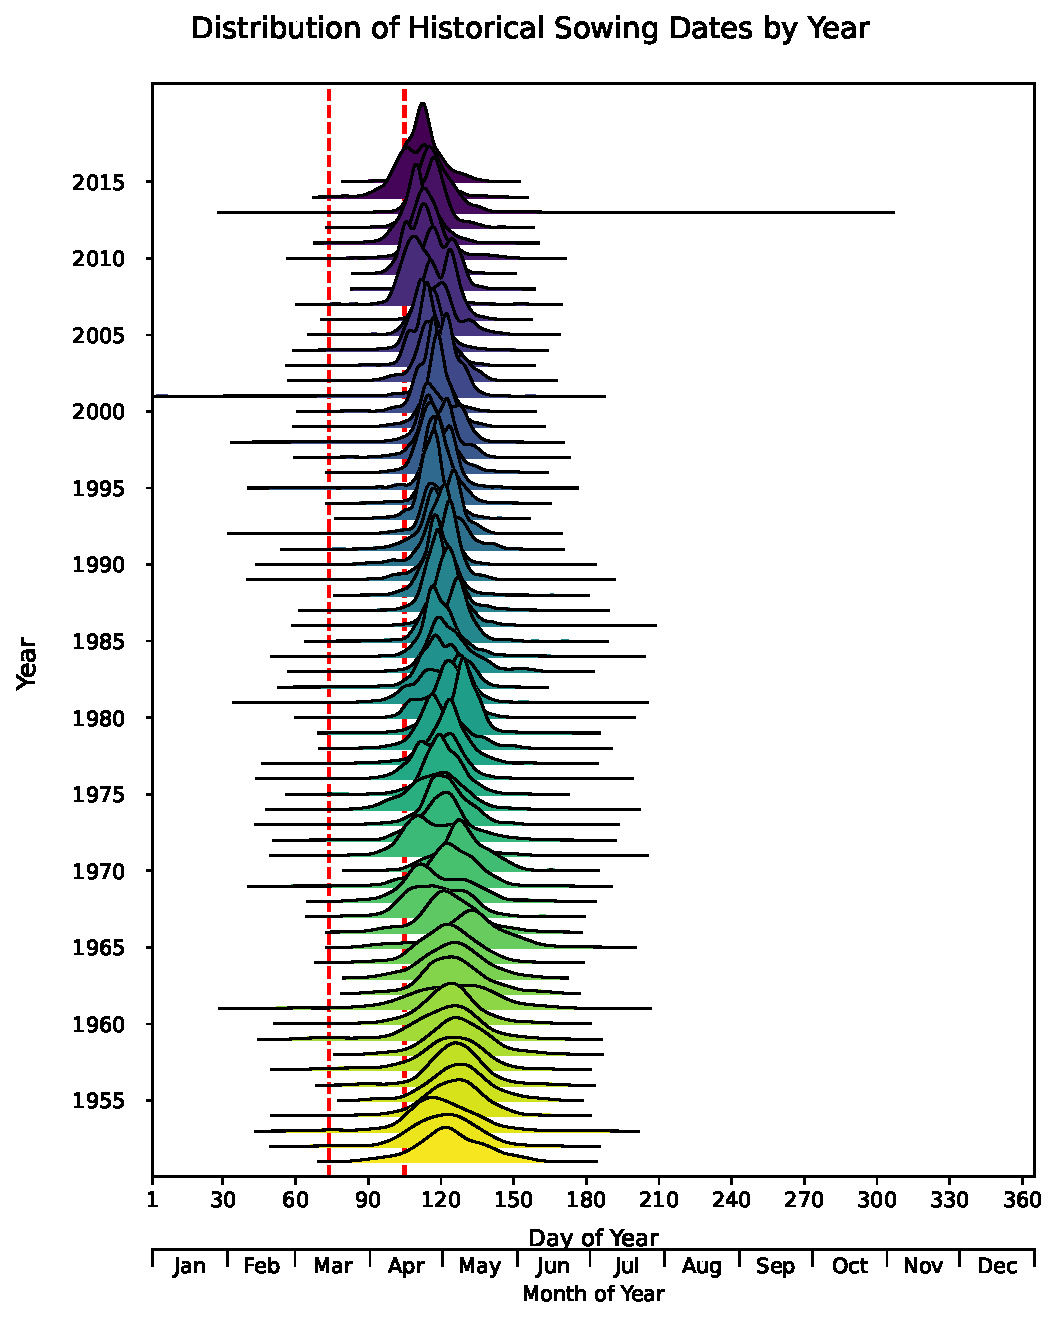
\includegraphics[height=0.9\textheight]{Sowing_dates_Distributions_VS_Crop_calendar-eps-converted-to.pdf}
		\column{0.5\textwidth}
			\begin{block}{Datos fenológicos}
				\begin{itemize}
					\item Calendario agrícola tomado del Joint Research Centre de la Unión Europea.
					\item Fechas de siembra tomadas de la plataforma Proyecto Fenología Paneuropea 725 (PEP725).
					\item Periodo 1951--2015.
					\item Tamaño de la muestra: 58115.
				\end{itemize}
			\end{block}
	\end{columns}
\end{frame}

\begin{frame}{Comparación 1951 vs. 2015}
	\vspace{-0.7cm}
	\centering
	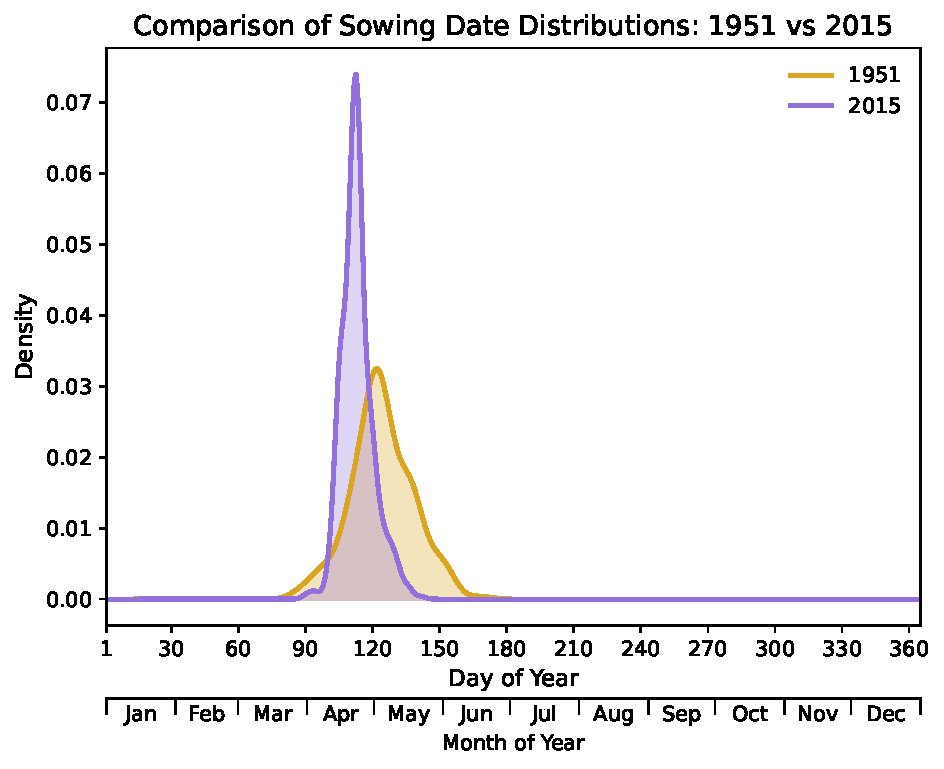
\includegraphics[height=0.9\textheight]{1951_VS_2015_Sowing_dates_Distributions.pdf}
\end{frame}

\begin{frame}{Comparaciones por año}
	\vspace{-0.7cm}
	\centering
	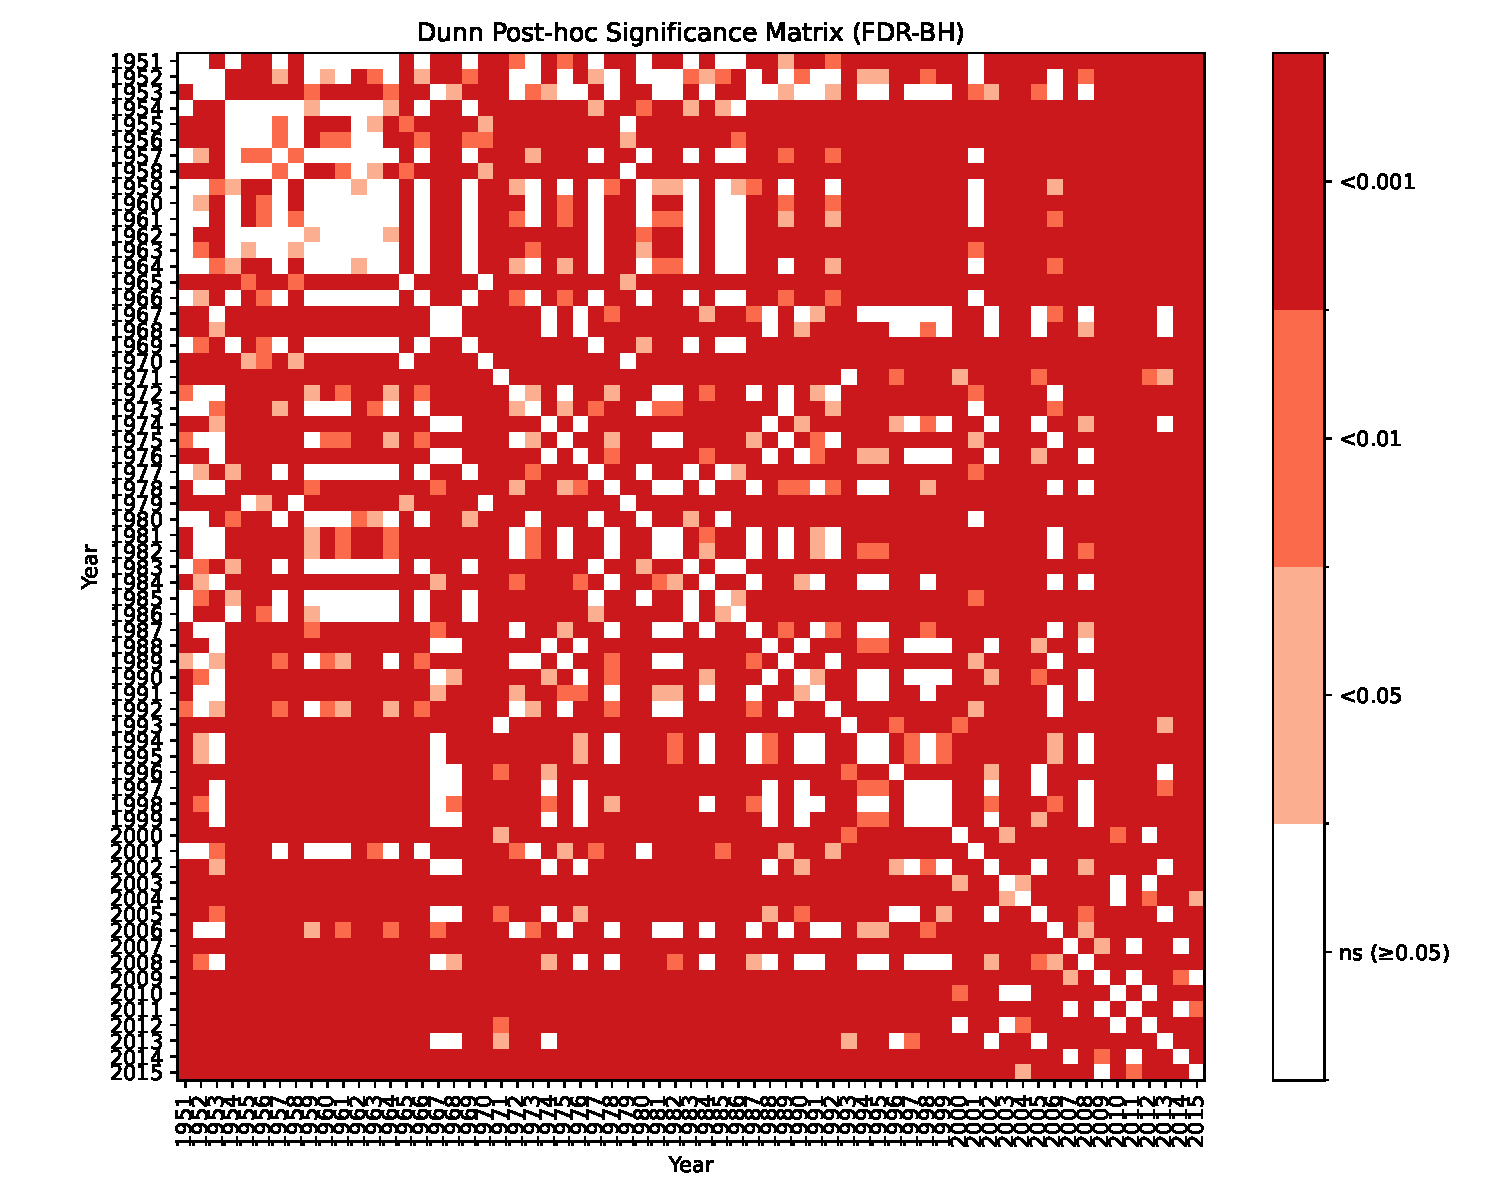
\includegraphics[height=0.9\textheight]{Historical_significance_matrix.pdf}
\end{frame}


\begin{frame}{Exploración de la hipótesis}
		\vspace*{-0.7cm}
		\begin{columns}
			\column{0.7\textwidth}
				\raggedleft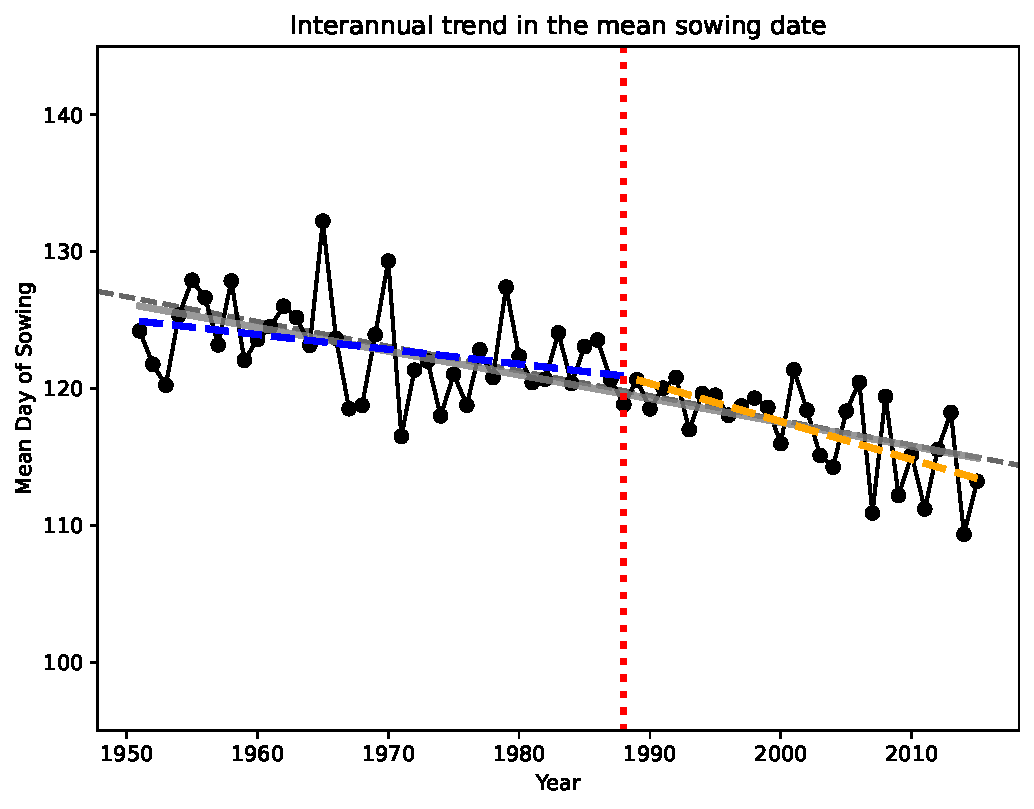
\includegraphics[height=0.9\textheight]{1988Break.pdf}
			\column{0.35\textwidth}
				\raggedright{El cambio estructural es consistente con lo previamente reportado por Chmielewski \textit{et al.} (2004); Menzel \textit{et al.} (2020); Reid \textit{et al.} (2015); Wu \textit{et al.} (2016).}
		\end{columns}
\end{frame}

\section*{Referencias}
\begin{frame}[allowframebreaks,noframenumbering]{Referencias}
	\vspace*{-1cm}
	\tiny
	\bibliography{Bibliografia.bib}
	\bibliographystyle{alpha}
	\nocite{*}
	%\printbibliography
\end{frame}

\section*{Gracias}
\begin{frame}[noframenumbering]
%\vspace{2cm}
     \begin{center}
	    \Huge{Gracias}
	\end{center}
\end{frame}    

\begin{frame}{Fechas de siembra}
	\vspace{-0.7cm}
	\centering
	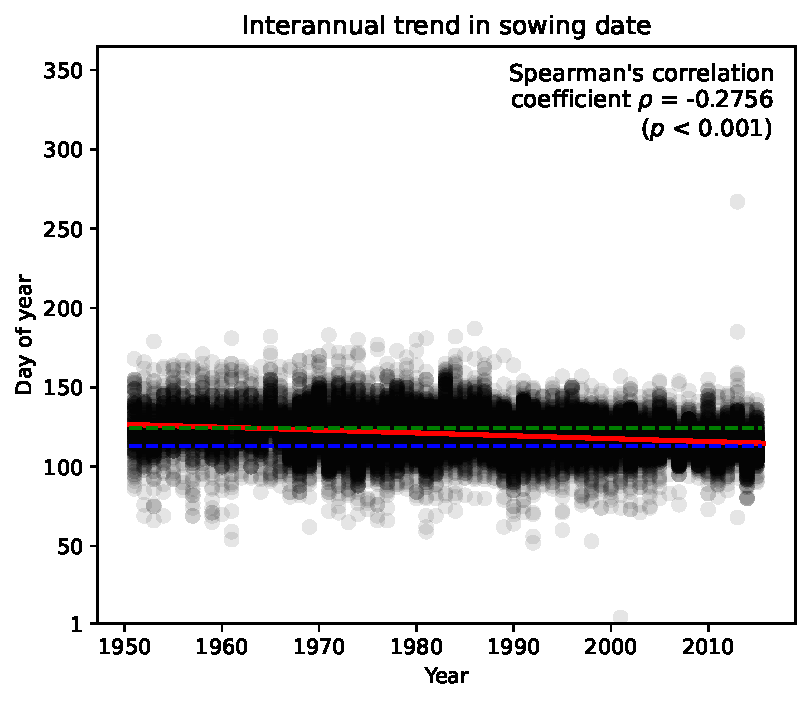
\includegraphics[height=0.9\textheight]{Interannual_trend.pdf}
\end{frame}


\begin{frame}{Variedades del maíz}
	\vspace{-0.7cm}
	\begin{columns}
		\column{0.5\textwidth}
			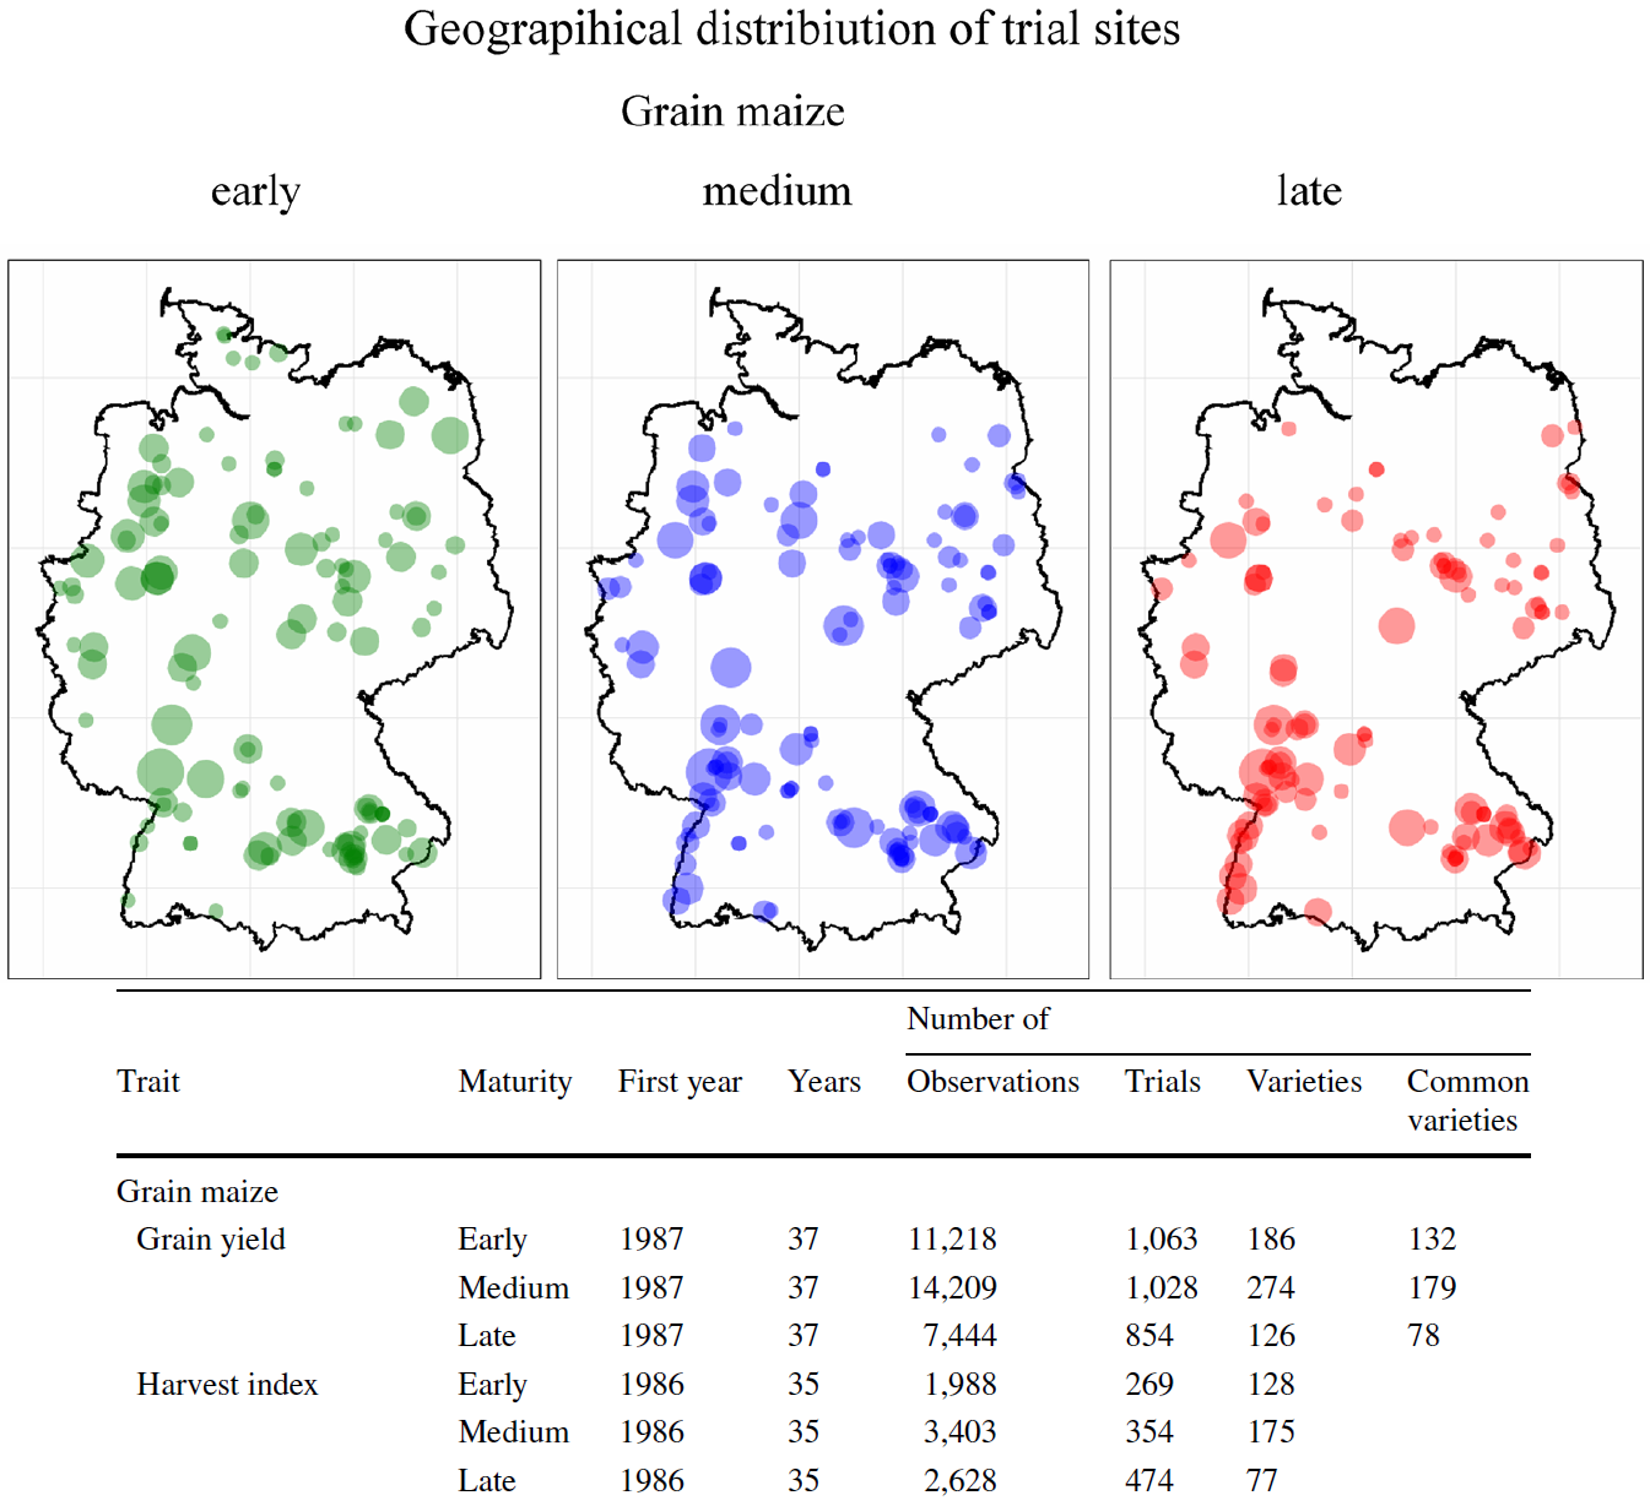
\includegraphics[width =\textwidth]{Effects of maize varieties.png}
		\column{0.5\textwidth}
		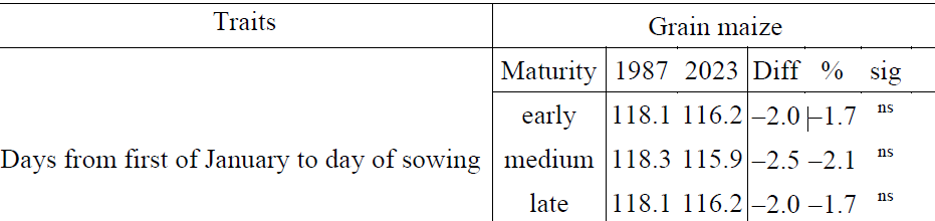
\includegraphics[width =\textwidth ]{Maize sowing varieties.png}
			Las distintas variedades de maíz comparten su respuesta a las condiciones de cultivo.
			
			{\scriptsize Fuente: Parent \textit{et al.} (2012); Sánchez \textit{et al.} (2014).}
			
		
			Las condiciones climáticas determinan la variedad a emplear.
			
			{\scriptsize Fuente: FAO (s.f.).}
	\end{columns}
	{\tiny Fuente: Laidig \textit{et al.} (2025). Breeding progress of grain and forage maize in long‑term variety trials compared to on‑farm yield development.}	
\end{frame}
    
 \begin{frame}{}
 	\centering
 	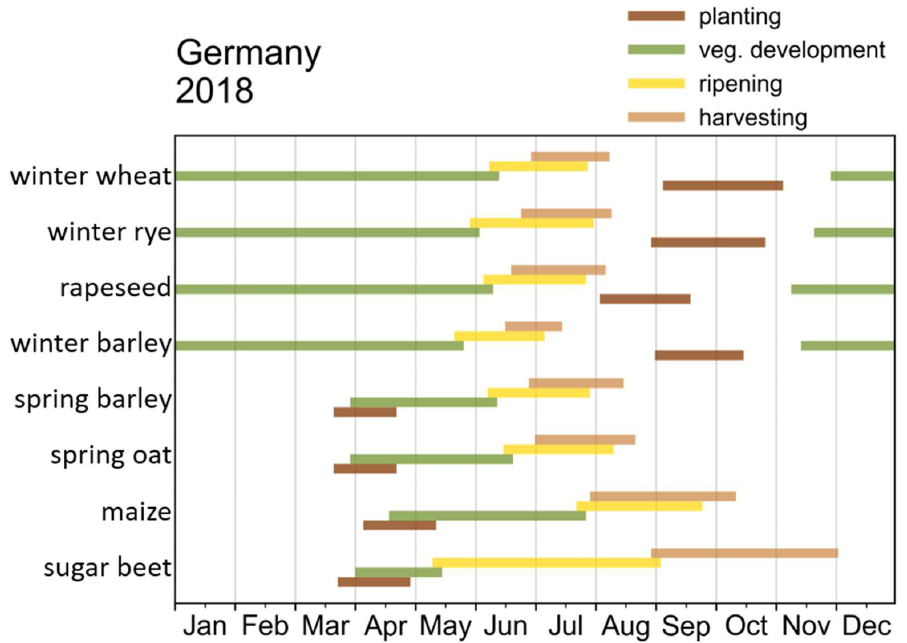
\includegraphics[height=0.5\textheight]{Crop calendar 2018.png}
 	
 	{\scriptsize Fuente: Asam \textit{et al.} (2022). Mapping Crop Types of Germany by Combining Temporal Statistical Metrics of Sentinel-1 and Sentinel-2 Time Series with LPIS Data.}
 	
 	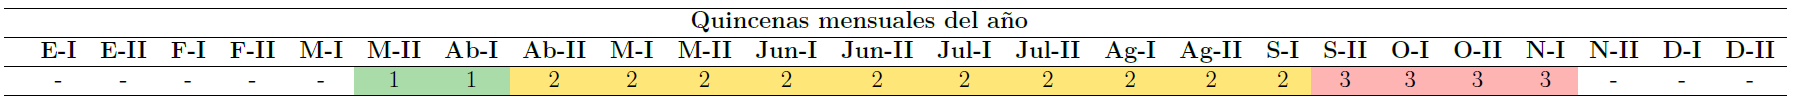
\includegraphics[width=\textwidth]{Crop calendar 2015.png}
 	
 	{\scriptsize Fuente: Joint Research Centre of the European Commission. (2026). Agri4cast Data Portal.}
 \end{frame}
\end{document}
